\documentclass[11pt,a4paper,titlepage,oneside,onecolumn]{article}

\usepackage{graphicx}
\usepackage{times}
%\usepackage{lucidabr}
%\usepackage{lucidamath}
%\usepackage{eurosym}
\usepackage{fancyhdr}
\usepackage{fancybox}
\usepackage{color}
\usepackage{colortbl}
\usepackage{tikz}
\usepackage[absolute,overlay]{textpos}
\usepackage{xcolor}
\usepackage{url}
\usepackage{wrapfig}

\usepackage[font={small,it},labelfont=bf]{caption}

\newcommand{\todo}[1]{\textcolor{red}{\textbf{TODO} #1}}

\pagestyle{headings}
%\pagestyle{fancy}

\linespread{1.4}

\setlength{\parskip}{5pt plus 2pt minus 1pt}
\setlength{\textwidth}{170mm}
\setlength{\textheight}{235mm}
\setlength{\evensidemargin}{0mm}
\setlength{\oddsidemargin}{0mm}
\setlength{\topmargin}{0mm}
\pagestyle{fancy}

\title{Visual Analysis of Protein-Protein Interactions}
\author{Assist. Prof.\ Dipl.-Ing.\ Dr.techn.\ Ivan Viola \and }

\begin{document}

\newpage\thispagestyle{empty}
\begin{center}
\large{\textbf{FWF-GA\v{C}R Project Proposal}} \\
between\\
TU Wien, 
Institute of Computer Graphics and Algorithms\\
Austria\\
and\\
Masaryk University Brno, 
Department of Computer Graphics and Design\\
and Department of Functional Genomics and Proteomics\\
Czech Republic\\
[4mm]\vfill
\textbf{\\\large{Visual Analysis of Protein-Protein Interactions}}
  
\begin{tabular}{c}
\hline
~~~~~~~~~~~~~~~~~~~~~~~~~~~~~~~~~~~~~~~~~~~~~~~~~~~~~~~~~~~~~~~~~~~~~~~~~~~~~~~~~~~~~~~~~~~~~~~~~~~~~~~~~~~~~~\\
\end{tabular}  

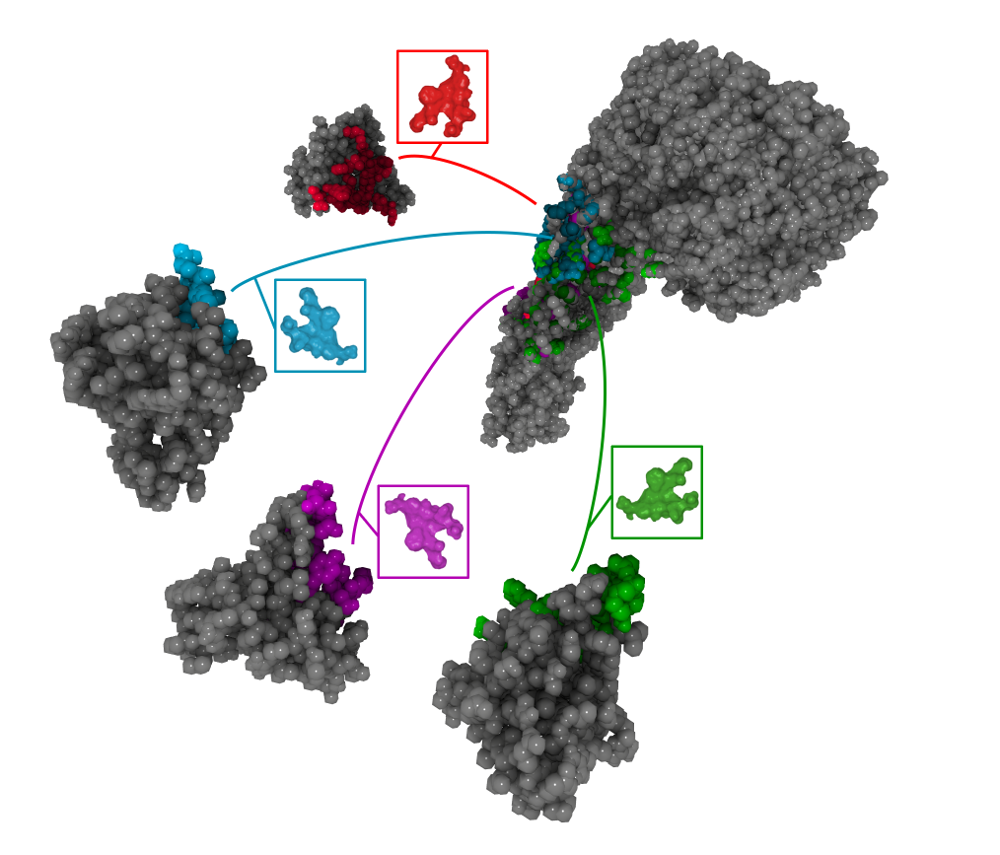
\includegraphics[width=0.78\textwidth]{pics/1aa.png}
%\todo{change image}

\normalsize{} 
submitted by\\
Assist. Prof. RNDr. Barbora Kozl\'{i}kov\'{a}, Ph.D., Assist. Prof.\ Dipl.-Ing.\ Dr.techn.\ Ivan Viola, \\ 
Assoc. Prof. Jan Pale\v{c}ek, Dr. rer. nat.%, RNDr. Jan By\v{s}ka, \\ 
%RNDr. Adam Jur\v{c}\'{i}k, TODO\\
\vfill
Vienna, Brno, March 2016
%\vspace{1cm}

%
\includegraphics[width=1.0\textwidth]{pics/podpisy.png}

\begin{tabular}{ccc}

%\begin{tabular}{c}
%\hline
%~~Dr. Ivan Viola~~
%\end{tabular} &

~~~~~~~~~~~~~~~~~~~~~~~~~~~~~~~~~~~~~~~~~~~~~~~~~~~~~~~~~~~~~~~~~~~~~~~~~~~~~~~~~~~~~~~~~~~~~~~~~~~~ &

%\begin{tabular}{c}
%\hline
%~~Dr. Ivan Viola~~
%\end{tabular} &

\end{tabular}

\end{center}



% TOC -------------------------------------------------------------------------
\newpage\thispagestyle{empty}
\linespread{1.0}
\begin{small}
\tableofcontents
\end{small}

% Body ------------------------------------------------------------------------
\newpage\setcounter{page}{1}
\begin{flushright}
    \shadowbox{
		\begin{minipage}[t]{8cm}
		\textbf{MISSION STATEMENT}\\
		\textit{To develop novel visualization technologies 
		that will revolutionarize protein-protein 
		interaction analysis workflows.}
		\end{minipage}
		}
\end{flushright}

%\begin{flushright}
%\fcolorbox{blue}{yellow}{\parbox{\textwidth}{%
%   \color{black}%
%	\begin{minipage}[c]{6cm}
%	\textbf{MISSION STATEMENT}\\
%   \textit{To develop novel visualization technologies \\
%  	that will revolutionarize protein-protein\\
%		interaction analysis workflows.}
%		\end{minipage}
%}}
%\end{flushright}

% Section: Introduction -------------------------------------------------------
\section{Introduction}
\label{sec:Introduction}
\vspace{-4mm}
Understanding the biological functions of proteins is a basal knowledge that contributes to advances in medicine, pharmaceutics, but also agriculture and even energy sectors. 
The ultimate goal of proteomic research is to describe functions of all protein complexes in cellular space and life time. 
Protein interaction patterns are, however, very complex, and revealing these is a challenging and time-consuming scientific process. 
Most of the proteins critical for cellular life act in a cooperative manner forming multiprotein complexes. 
It is estimated that about 800 complexes exist in just one yeast cell.
All complexes are composed of subunits which constitute the complex via protein-protein interactions.
The main goal in studying such protein-protein interactions is to identify an appropriate spatial conformation of interacting proteins (see Figure \ref{fig:dock}). 
These studies span from investigating interactions between two protein structures to exploring large multi-molecular complexes.
Every subunit of such complexes makes its contacts with neighboring subunits under a specific spatial orientation that is critical for the function of the whole complex.


Protein structures studied with respect to their mutual interactions are primarily defined by the sequences of amino acids. 
This 1D sequential information does not give any explicit information about the spatial conformation of the protein chain.
However, for studying interactions between two or more proteins, the knowledge of the 3D protein structure is crucial because it reveals the potential contact surfaces between proteins.
The process of creating the protein spatial conformation is called folding.%For one protein sequence the folding usually produces several possible spatial conformations which have to be further studied and evaluated by a domain expert. 
%The domain expert selects one or a small number of the most probable spatial conformations, which will serve as input for the following phases.

Subsequently, the set of these 3D conformations of proteins is tested for their mutual interaction. 
This process is called \textit{molecular docking}. 
Existing approaches calculate a mutual conformation of two interacting proteins and suggest several most probable contact zones~\cite{huang}. 
The subsequent task is to evaluate the biochemical relevance of these results. 
Such an evaluation is nowadays performed using manual comparisons or utilizing traditional 3D visualization methods which have been used in molecular visualization for decades.
\setlength\intextsep{0pt}
\begin{wrapfigure}{l}{0.6\textwidth}
  \vspace{-5mm}
	\begin{center}
  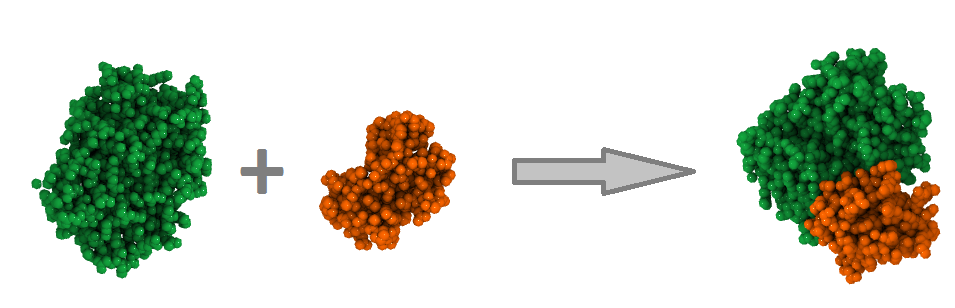
\includegraphics[width=0.6\textwidth]{pics/docking.png}
	\end{center}
	\vspace{-5mm}
  \caption{Two protein chains and their mutual interaction.}
  \label{fig:dock}
\end{wrapfigure}
The main limitations of the existing methods are the occlusion caused by the 3D environment, hidden contact zones, and high overlaps when comparing more conformations (see Figure~\ref{fig:problem}).

\setlength\intextsep{0pt}
\begin{wrapfigure}{l}{0.4\textwidth}
\vspace{-5mm}
\begin{center}
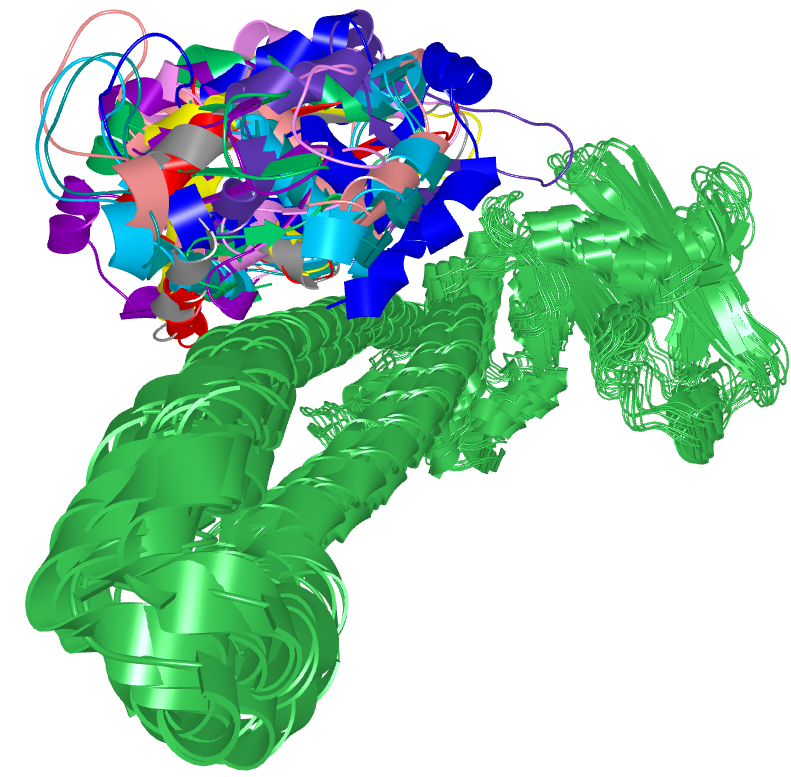
\includegraphics[width=0.4\textwidth]{pics/problem.png}
\end{center}
\vspace{-5mm}
\caption{Superposition of several possible conformations between two proteins visualized using a traditional cartoon method. The set of green protein instances corresponds to one of the proteins in the interaction, the colored components represent the second protein in different conformations. Due to the high visual overlap, this visualization does not allow a clear comparison.}
\label{fig:problem}
\end{wrapfigure}

While there are many existing algorithms searching for protein-protein docking, researchers suffer from a lack of appropriate solutions for visual representations, explorations, and comparisons of the results. 
A similar situation holds for the already determined contacts between proteins which are available, e.g., in the PDBsum database~\cite{pdbsum}.
The database currently contains thousands of entries for protein-protein interfaces which capture the 3D mutual orientation of the docked proteins using JMol~\cite{jmol} and provides the users with an abstracted static representation of the contact zones (see Figure~\ref{fig:pdbsum}).

\setlength\intextsep{0pt}
\begin{figure}[bt]
  \vspace{-5mm}
  \centering
  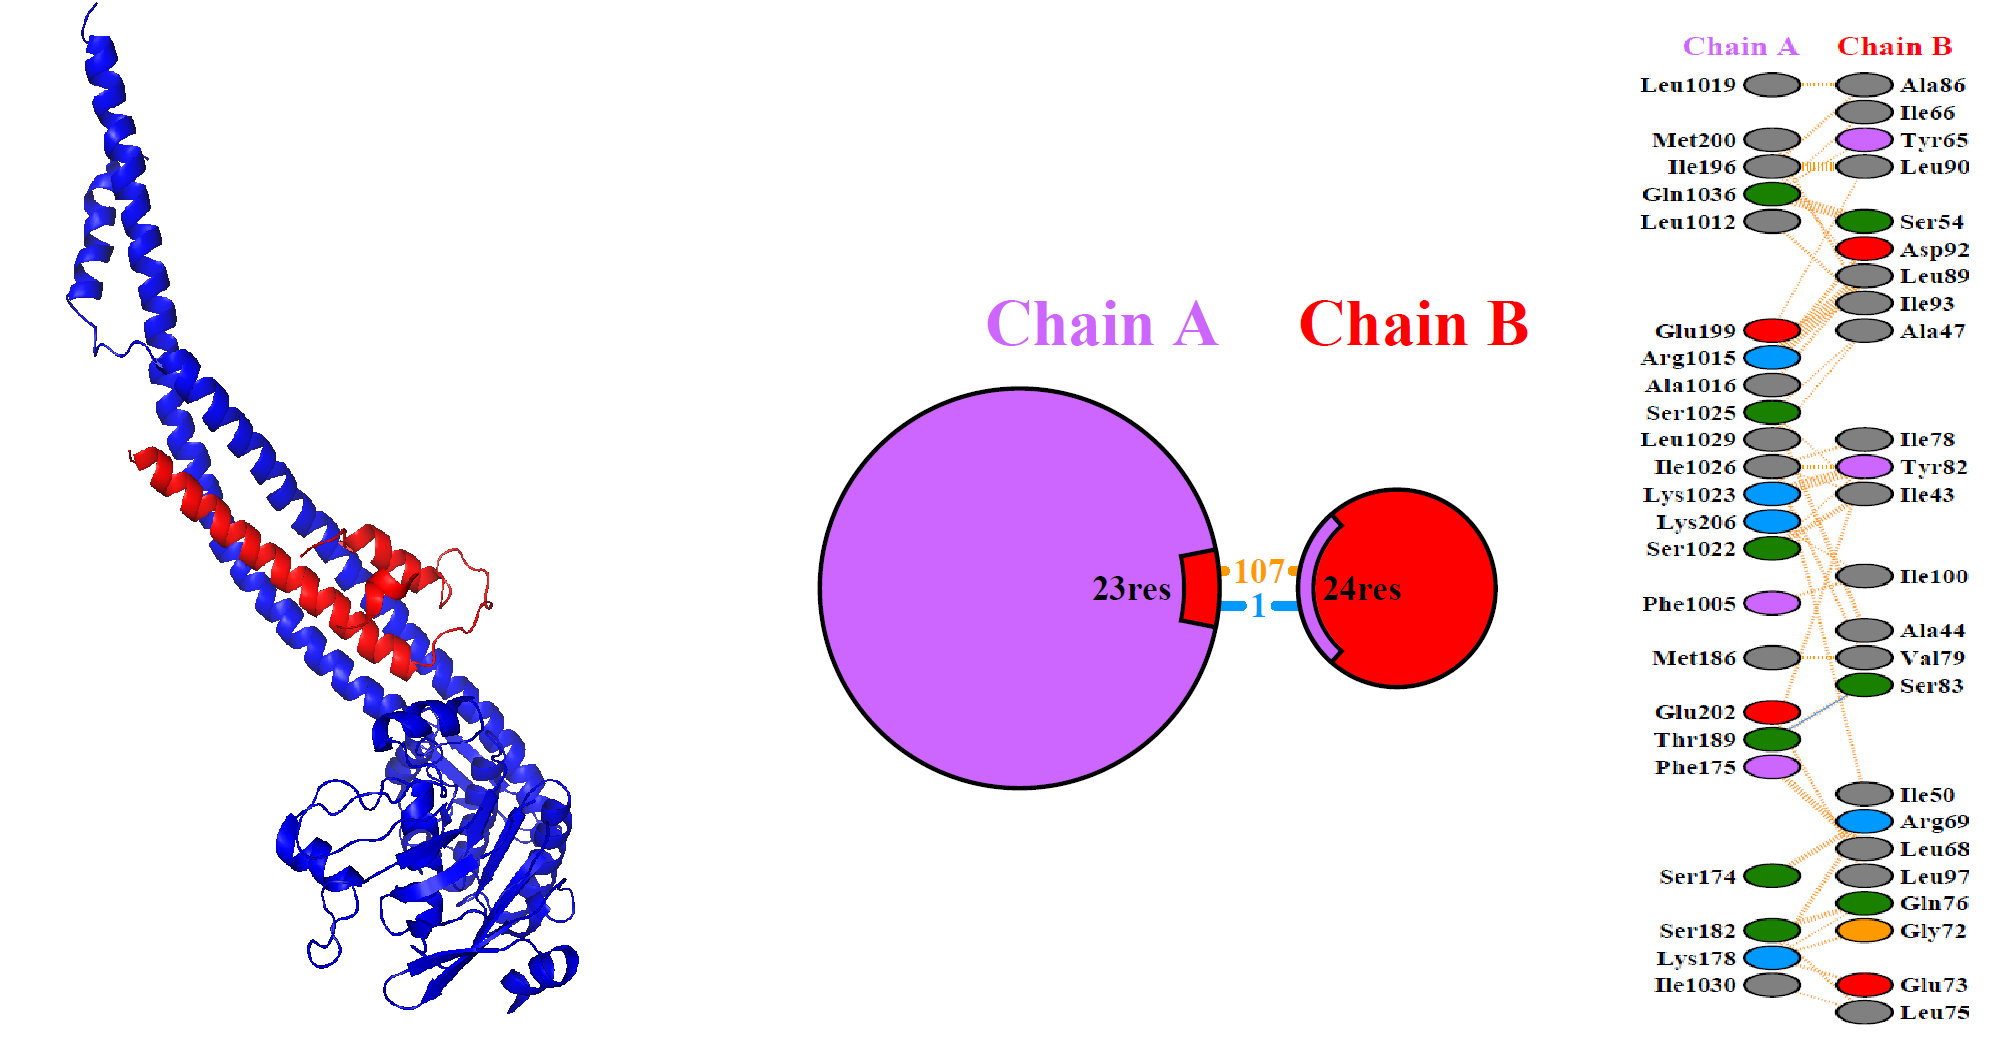
\includegraphics[width=0.8\textwidth]{pics/pdbsum3.png}
  \vspace{-5mm}
	\caption{Existing visual representations of the crystal structure of complex SMC3-Scc1 with ID 4UX3 stored in the PDBsum database. Left: 3D structure, middle: abstracted representation of the contact zones between the chains, right: detailed interactions between individual amino acids as represented in the PDBsum database.}
  \label{fig:pdbsum}
\end{figure}

However, the existing visual representations do not allow the user to interactively explore the contact zones nor to compare different protein-protein interfaces.
%The latter is helpful mainly in cases when the biochemists are searching for a proper contact zone for still unexplored combination of proteins but the interaction of some of these proteins with other ones was already revealed, annotated, and stored in the database. 
The information from the existing databases can serve as a reference or guidance and the visual comparison is a necessity.
This functionality is not available in the existing visualization tools.
Current visual workflows employ the widely used tools for molecular visualization such as PyMol~\cite{pymol} or VMD~\cite{VMD} which are targeting a broad user base and do not focus on specialized visualizations for a given task.
In consequence, the usage of general techniques is often impractical as it does not  provide the necessary information to support a particular workflow.
An example can be the superposition of several possible conformations of two interacting proteins illustrated in Figure~\ref{fig:problem}.
In this case, the proteins are represented by the cartoon visualization method and the colored proteins represent different possible positions with respect to the green (aligned) ones.
It is obvious that such a cluttered representation cannot be used for an intuitive comparison of individual solutions.



%After the comparison stage, the set of the biochemically most relevant docking results usually contains several solutions.
%The contact zones of these results can be further modified in order to find the most critical amino acid(s) for the particular protein-protein interaction. 
%Such crucial amino acids are called \textit{hot spots} and the process of amino acid modification is called \textit{mutagenesis}. 
%It enables one amino acid in the protein chain to be replaced by another one in order to change the protein properties.
%In-silico identification and mutagenesis of one crucial hot spot of each of the proposed docking models will provide a major target for the experimental mutagenesis approach. 
%This can significantly reduce the number of the real protein mutants required for the determination of the real contact zone.


With respect to the docking problem, the current solutions focus mainly on searching for possible interactions between two proteins.
However, proteins can also form more complicated \textit{complexes of proteins} where several protein structures interact with each other.
For this process, called \textit{multidocking}, the set of possible contact zones increases exponentially. 
In this case existing visualization tools do not even offer a minimally sufficient solution, and research for effective visual explorations, comparisons, and ranking is urgently needed.

%The complexity of the described research area is enormous, and suitable visualization technology does not exist to this date. 
%Technologies which are described in the molecular visualization scientific literature tackle the protein-protein interaction problem very rarely. 
%They mostly deal with ligand docking, which investigates the interaction of a small molecule, usually a drug, with the host protein macromolecule. 
%It is not obvious how existing visualization technology can be adapted to the delineated problem of protein-protein interactions.
%A substantial research effort is expected in order to investigate novel visualization techniques that could aid the analytic workflow (see Figure \ref{fig:workflow}). 

\setlength\intextsep{0pt}
\begin{wrapfigure}{l}{0.5\textwidth}
  \begin{center}
  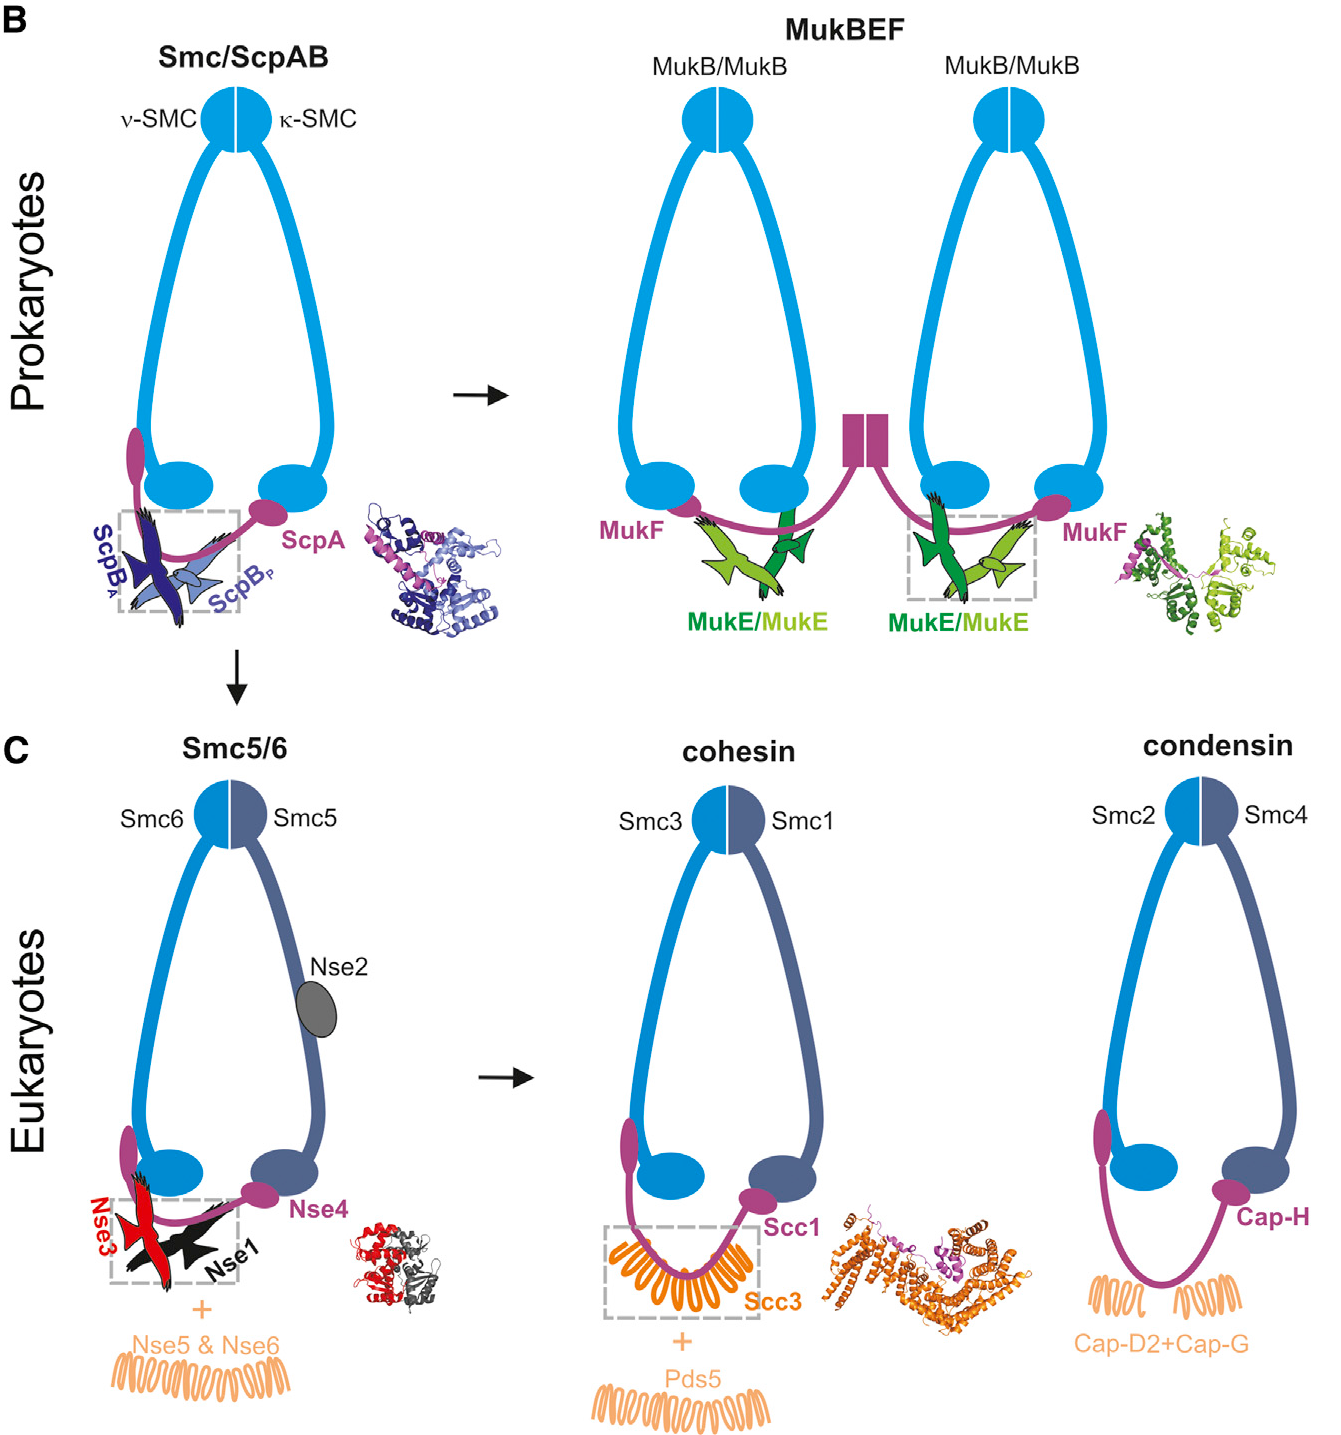
\includegraphics[width=0.5\textwidth,height=0.48\textwidth]{pics/telomer.png}
	\end{center}
	\vspace{-20pt}
  \caption{Architecture and composition of SMC complexes (taken from Pale\v{c}ek and Gruber~\cite{Palecek2015}). These complexes will serve in the evaluation of the usability of our proposed visualizations and visual analysis tools.}
  \label{fig:telomere}
\end{wrapfigure}

As a part of the research project, the novel visualization technology will be tested with the ongoing biological research at the Department of Functional Genomics and Proteomics (DFGP), located at the Faculty of Science at the Masaryk University in Brno. 
The focus of interest of researchers at DFGP is on SMC (structure maintenance of chromosome), telomere-associated, and other chromatin complexes. 
The SMC complexes are key players in chromatin organization and dynamics (e.g., the condensin complex ensures a proper condensation of chromosomes -- see Figure~\ref{fig:telomere} taken from Pale\v{c}ek and Gruber~\cite{Palecek2015}) and are the main focus of the Pale\v{c}ek's group.
Pale\v{c}ek's group (group of Structural Proteins of Eukaryotic Chromosomes; SPEC) group analyzes the architecture and function of such complexes using a variety of experimental approaches. 
Their goal is to uncover the way how the subunits of these complexes interact with each other and execute unique function(s) of these complexes. 
Therefore, a visual representation of such information is highly beneficial because it helps to reveal the spatial relationships between the subunits in an intuitive way.



\section{Objectives}
\vspace{-4mm}
The objectives of the project follow its two stages which are depicted in Figure~\ref{fig:system}.
The first objective is to design novel visualization metaphors supporting particular tasks and to build a system for visual analysis combining the proposed visualization methods into an intuitive and interactive environment.
The second objective is related with the fact that visual analytics frameworks are currently being developed in many fields of sciences to support the analytical workkflows of specialists. 

\setlength\intextsep{0pt}
\begin{wrapfigure}{r}{0.5\textwidth}
\vspace{-8mm}
\begin{center}
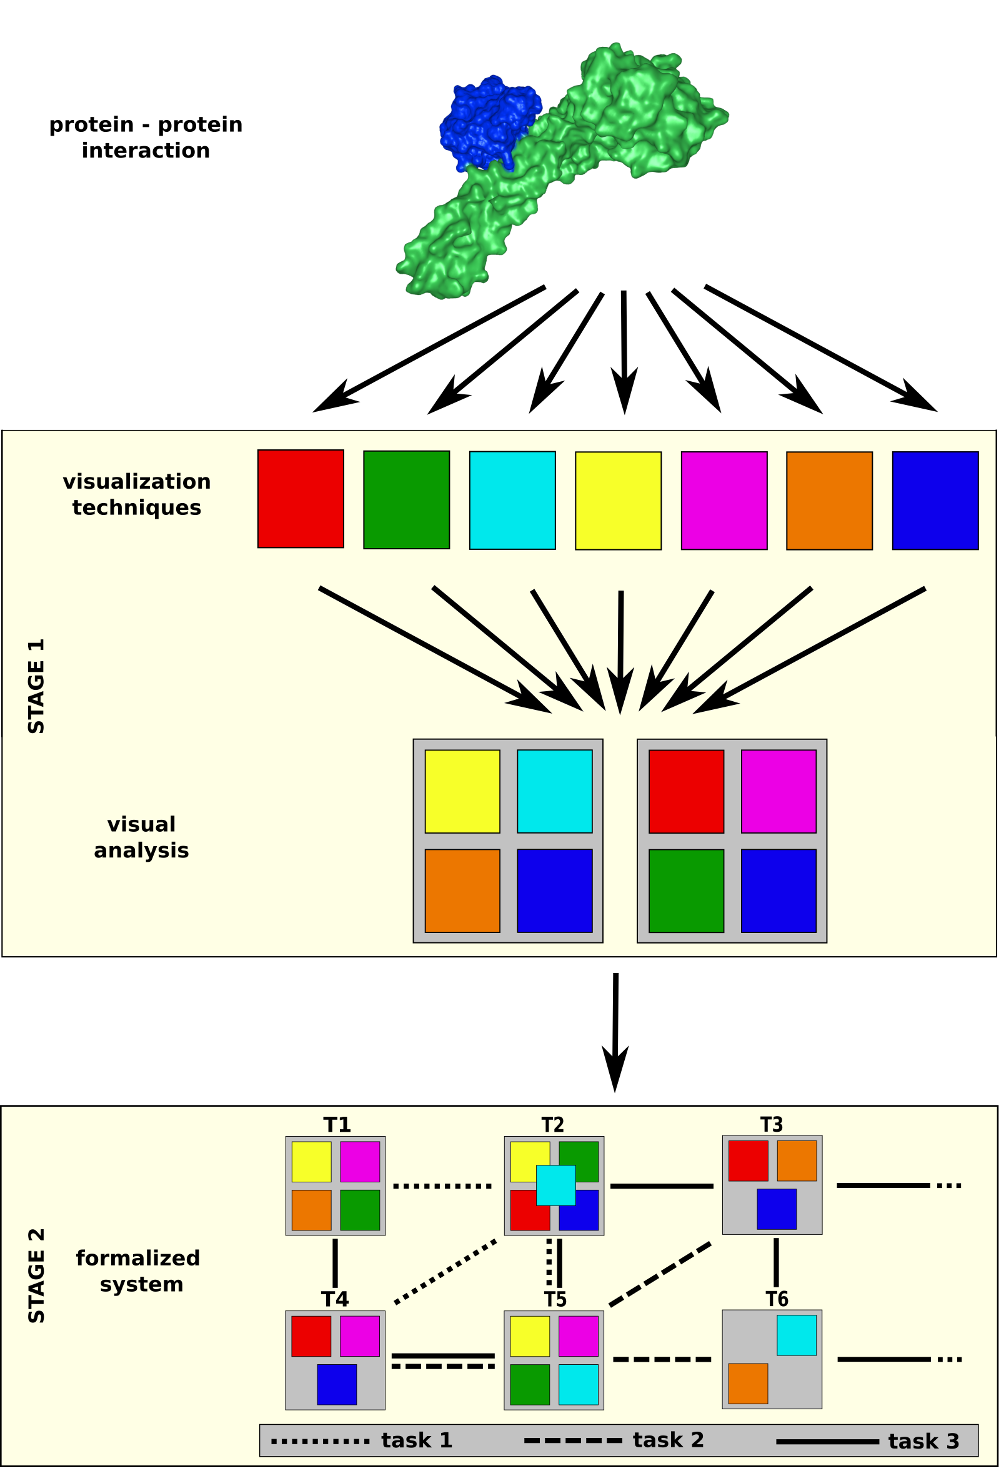
\includegraphics[width=0.5\textwidth,height=0.7\textwidth]{pics/systemsmall.png}
\end{center}
\vspace{-5mm}
\caption{Overview of the project outline. In Stage 1 we will focus on designing specific visualizations for given tasks and building visual analysis systems consisting of these visualizations. Stage 2 proposes a formalized model of the visual analysis systems which will focus on specific tasks Ti.}
\label{fig:system}
\end{wrapfigure}
However, they lack a systematic formalization of the design choices.
It is the case of our underlying domain problem as well. 
We want to use this use case for advancing conceptual level of visual analytics by proposing a formalization of the theory for visual analytics frameworks design given a specific set of data and analytical goals.

%The potential impact of the outcome of this project for the scientific discipline of structural biology is substantial.
%To enable efficient visual comparison of complex protein structures, we will develop a semantically-driven flattening approaches so that important aspects of an entire surface of particular 3D structure will be described in one image. Furthermore, we will link or directly integrate meaningful information visualization techniques such as matrices, ranking representations, or hypergraphics with spatial visualization, resulting into comprehensive heterogeneous visualizations able to communicate a large picture of multiple aspects of the underlying data. We will develop new visual guidance techniques based on controlling movement of molecular dynamics simulations driven by domain semantics, propose new suggestive visualizations that will help to propose the most appropriate candidate amino acids for mutagenesis, and multidocking will be guided so that the analyst is not lost in the complexity and clearly understands which multidocking conformations are physically plausible.


%\begin{figure}[t]
%  \centering
%  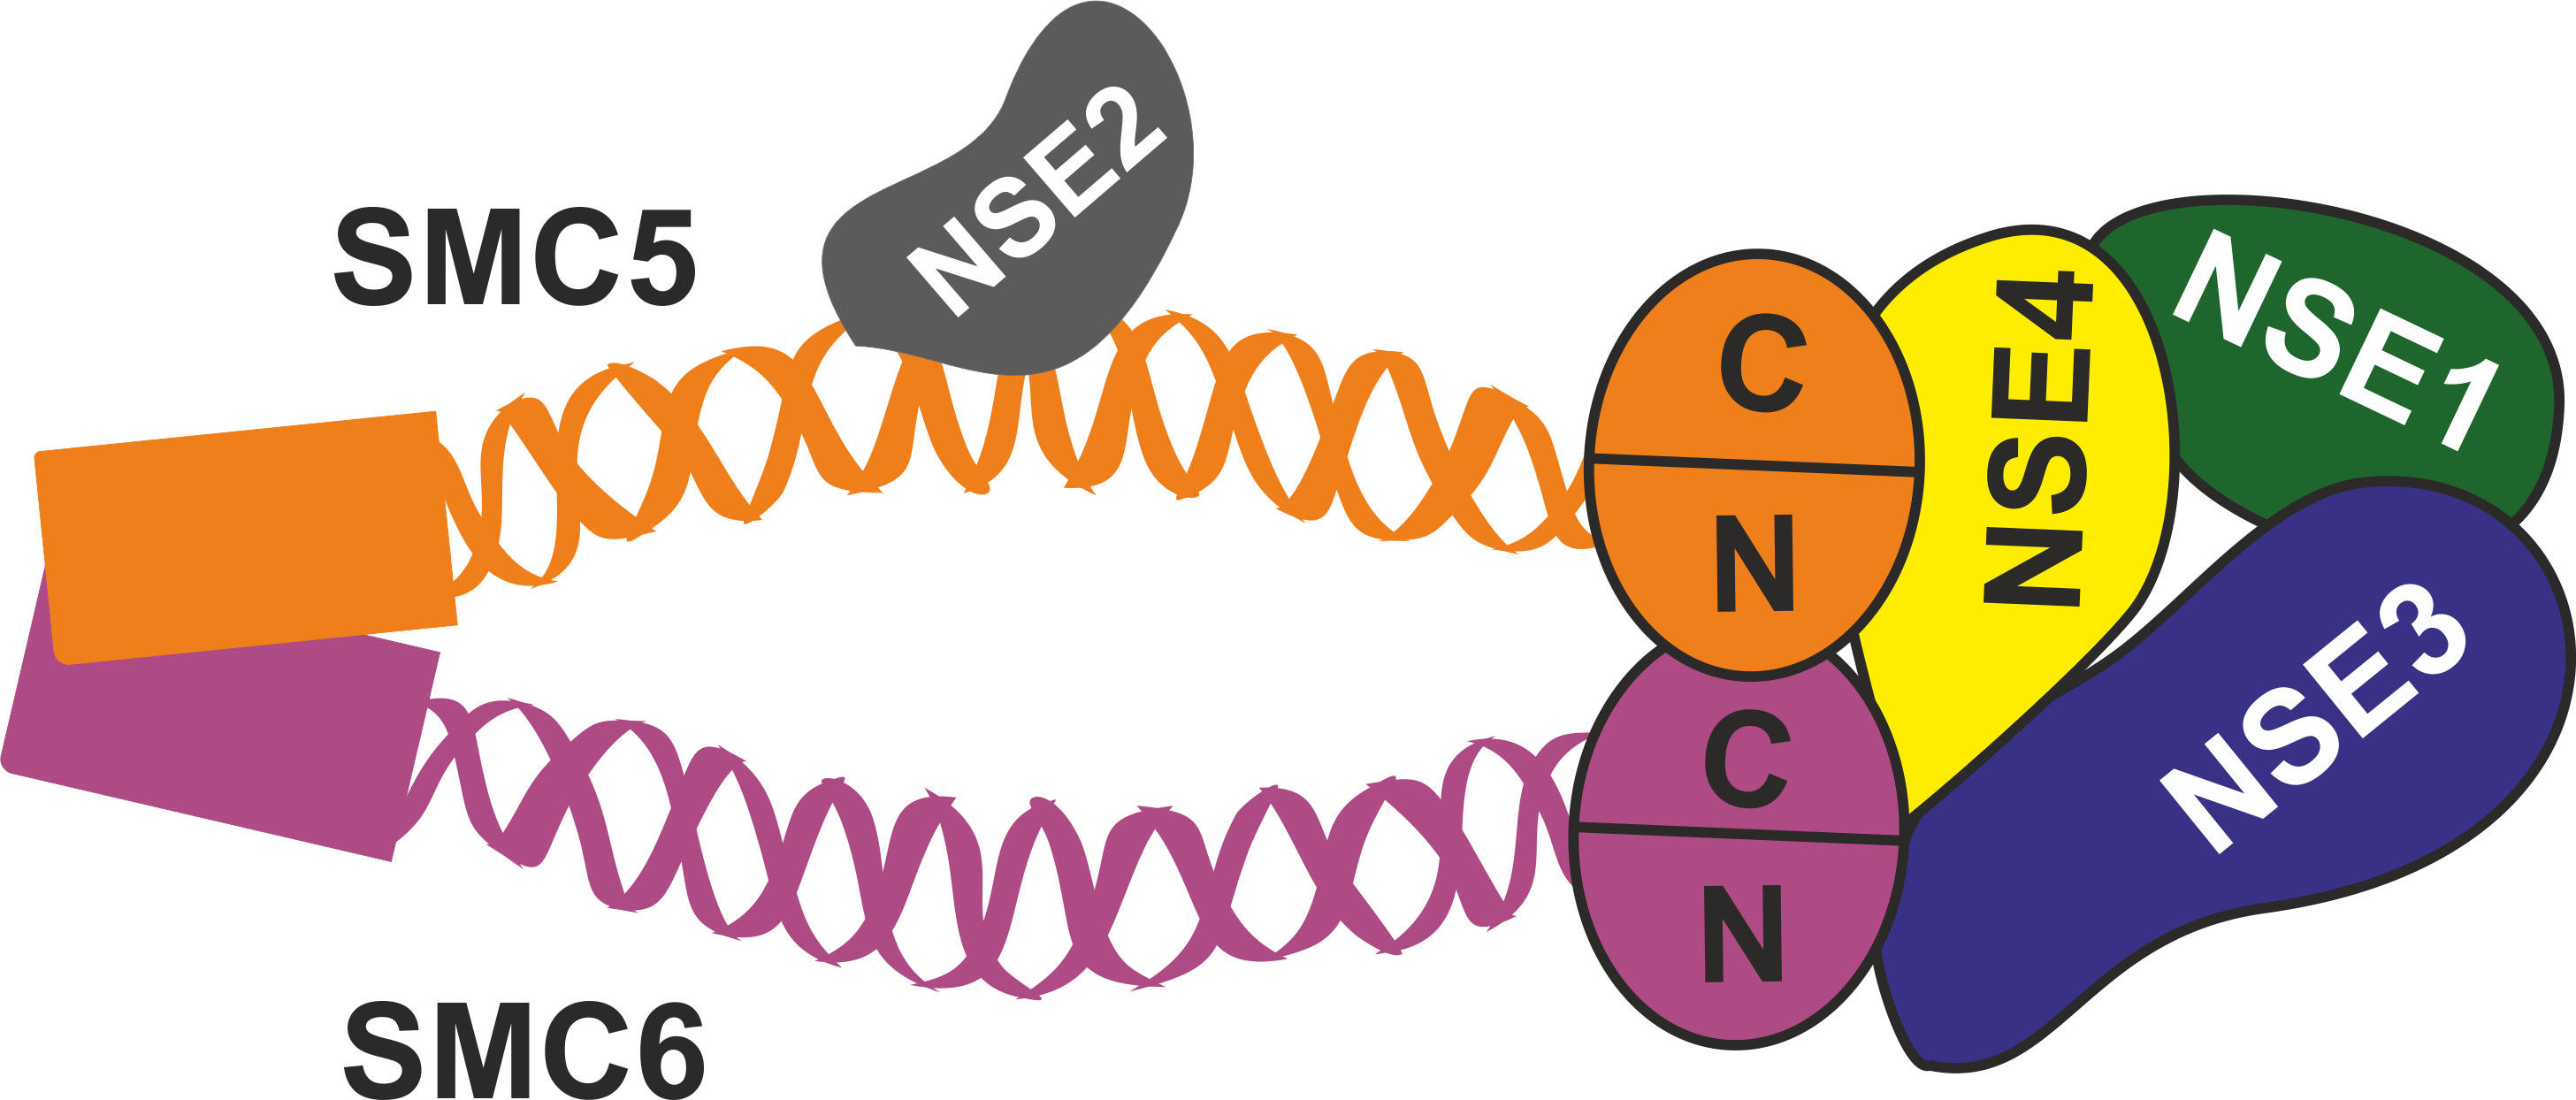
\includegraphics[width=0.4\textwidth]{pics/smc.png}
%  \caption{Architecture of the SMC5/6 complex.}
%  \label{fig:complex}
%\end{figure}
% Section: State of the Art ---------------------------------------------------
\section{State of the Art}
\label{sec:StateOfTheArt}
\vspace{-4mm}
The previous work related to the scope of our project consists of several parts. 
First, we briefly describe the basic principles of existing solutions for the computational analysis of protein structures, including protein-protein interactions. 
Then we review the existing approaches for the visualization of protein surfaces as the contact zones between proteins can be visualized as surfaces in 3D.
This is followed by surveying methods for an interactive visual analysis and visual guidance through large molecular systems, which combine several representations in order to get a comprehensive view on the whole system. 

\subsection{Computational Analysis of Proteins}
\vspace{-4mm}
The spatial conformation of a protein greatly influences its reactivity and properties, thus many publications are related to the geometrical analysis of protein structure. 
Proteins can react with other structures, such as small molecules or other proteins, via chemical reactions or interactions occurring deeply inside the protein or on the protein surface.
In the first case, the protein inner void space gives the opportunity for small molecules to enter the protein and perform a chemical reaction. 
The inner voids (called cavities) along with their entrance paths (tunnels, channels, or pores), which are traversed by small molecules, have been intensively studied in the last decade.   
Most of the existing algorithms for the detection of entrance paths are based on simple Voronoi diagrams \cite{caver,mole,molaxis} or Voronoi diagrams of spheres \cite{Kim,Lindow2011}. Benkaidali et al. \cite{Benkaidali} presented an alternative method using modified alpha shapes. 
In 2013, Krone et al. \cite{Krone2013} published another approach for the detection of cavities, channels, and pockets, which was based on the concept of ambient occlusion. 
Krone et al. \cite{Krone2011} further introduced a method for the detection and interactive exploration of protein cavities. 
Lindow et al. \cite{Lindow2012} presented a Voronoi based algorithm for the computation of cavities and channels from molecular dynamics trajectories. 
Their dynamic channels are computed by analyzing the temporal evolution of components of the cavity structure.

If a protein interacts with another protein structure, the computational analysis solves the problem of detecting interaction contact zones on the surfaces of these proteins. 
The currently existing search strategies for protein-protein docking can be divided into four categories. 
The first category consists of methods using an exhaustive global search which requires enormous computational resources.
The other categories use local shape feature matching, randomized search, or post-docking approaches employing advanced scoring functions or consider protein flexibility. Details about these approaches as well as a list of existing solutions can be found in the survey of Huang \cite{huang}.

\setlength\intextsep{0pt}
\begin{wrapfigure}{l}{0.49\textwidth}
\vspace{-5mm}
  \begin{center}
  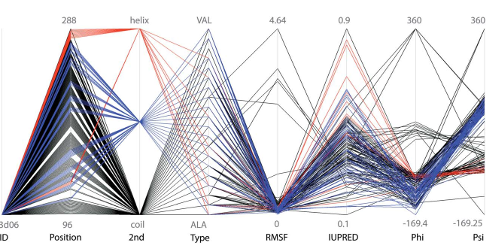
\includegraphics[width=0.49\textwidth]{pics/parallel2.png}
	\end{center}
\vspace{-5mm}
  \caption{Parallel coordinates showing different amino acid attributes. Each amino acid is represented as a polyline. Image taken from Krone et al.~\cite{Krone2014}.}
  \label{fig:parallel}
\end{wrapfigure}
Existing visual representations of computed structures (pathways or contact zones) mostly deal with their 3D spatial arrangement. 
However, such a 3D visualization is rather limited, mainly with respect to depicting many properties (physico-chemical, geometric) of the amino acids forming the pathways or contact zones. In such cases an abstracted representation is more appropriate. 
An example of this was presented by Heinrich et al.~\cite{Heinrich2014} where the authors use parallel coordinates to convey many attributes of amino acids (see Figure~\ref{fig:parallel}). 
Furthermore, when dealing with several proteins at once, the visual comparison of results in 3D is impossible to reach in a clear and comprehensible way.  

\subsection{Visualization of a Protein Surface}
\vspace{-4mm}
The protein surface plays a crucial role in interactions with the outer environment, including other molecules. 
In case of protein-protein interactions, the most important parts of the proteins are the mutual contact zones. 
These zones can be represented by one of the traditional models for visualization of their amino acids (e.g., space-filling model). 
One of the most common methods is to represent the contact zone by its surface. 
%In fact, it is a part of the entire protein surface which has been studied and visualized for decades.

There are many publications focusing on the visualization of molecular surfaces.
Here we will mention only the latest results in this field.
In 2012, Parulek and Viola~\cite{ParulekViola2012} presented the first ray-casting of the so called solvent excluded surface that does not need a precomputation of the analytical description of the surface.
They use a modified sphere tracing and directly compute the implicit description of the surface based on the local neighborhood of a ray.   
In contrast to these direct ray-casting approaches, Decherchi and Rocchia~\cite{Decherchi2013} presented a new triangulation method based on ray-casting. 
It performs ray-casting through a 3D grid from which the surface is extracted using the Marching Cubes algorithm. 

%Detected pathways are typically visualized as a set of intersecting spheres positioned on the tunnel centerline. 
%Such a representation is supported also by other molecular visualization tools, e.g., PyMol \cite{pymol} or VMD \cite{VMD}.
%By\v{s}ka et al. \cite{byska} introduced the concept of asymmetric tunnels which captures the real tunnel shape much better.
%The asymmetric tunnels are computed combining a Voronoi diagram and a grid based approach.
%An asymmetric representation is achieved also by methods introduced by Lindow et al. \cite{Lindow2012,Lindow2013}.

In our case the surface of a protein can be divided into two parts -- contact zone (focus) and the remaining part (context). 
The contact zone has been studied in a method published by Lee and Varshney~\cite{Lee2006}. 
Their approach uses the hypothesis that the intermolecular volume and the area between docked molecules is useful as a measure of the shape complementarity. 
Therefore they propose an algorithm for the interactive computation of a so called intermolecular negative volume. In combination with dedicated visual representations (see Figure~\ref{fig:varshney}), it can serve the domain experts as an interactive tool for studying possible docking conformations.

\setlength\intextsep{0pt}
\begin{wrapfigure}{l}{0.48\textwidth}
\vspace{-5mm}
  \begin{center}
  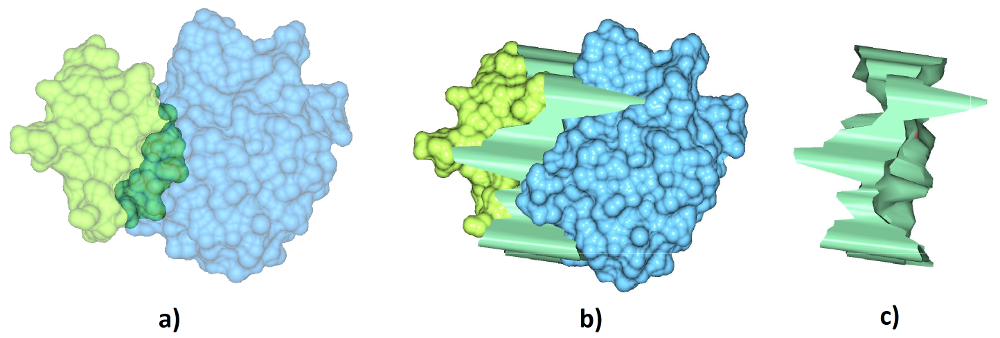
\includegraphics[width=0.48\textwidth]{pics/varshney2.png}
	\end{center}
\vspace{-5mm}
  \caption{Visual representations of the contact zones proposed by Lee and Varshney. a) Translucent surfaces, b) Intermolecular negative volume between molecules, c) Intermolecular volume only. Image taken from Lee and Varshney~\cite{Lee2006}}.
\vspace{-5mm}
  \label{fig:varshney}
\end{wrapfigure}
The context part can be represented using some level of abstraction. Cipriano and Gleicher \cite{cipriano} presented a visualization technique which provides an abstracted view of the shape of molecules.
Their approach suppresses small details to facilitate rapid comprehension but marks the location of significant but removed features so they remain perceivable.

Along with the algorithms and techniques for both analysis and visualization of macromolecules, several tools integrating individual techniques emerged. 
Some of them are quite widespread and currently serve the chemists in the visualization of results from various analyses. 
The PyMol software tool \cite{pymol} enables the users to integrate and render the results of their own analyses by employing Python scripting. 
The VMD tool \cite{VMD} is a molecular visualization program which enables displaying, animating, and analyzing large biomolecular systems. 
UCSF Chimera \cite{chimera} is an application for the interactive visualization and analysis of molecular structures and related data. 

%\begin{wrapfigure}{r}{0.6\textwidth}
%  \begin{center}
%  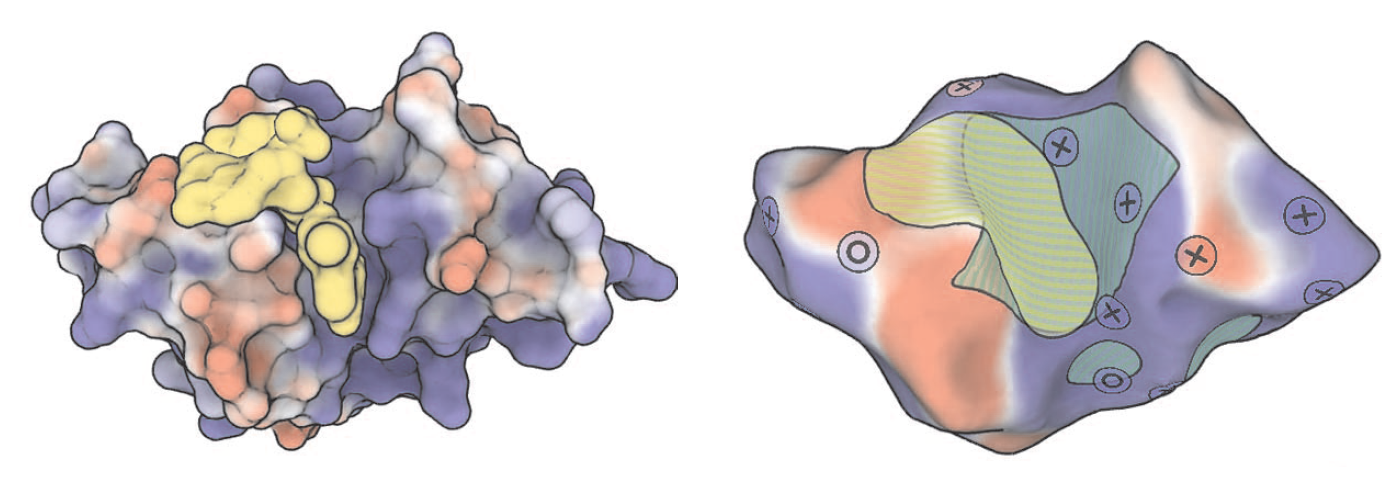
\includegraphics[width=0.6\textwidth]{pics/abstract.png}
%	\end{center}
%  \caption{Protein surface and its abstracted representation smoothing the surface and marking the significant locations using glyphs \cite{cipriano}.}
%  \label{cipriano}
%\end{wrapfigure}

\subsection{Interactive Visual Analysis and Visual Guidance}
\vspace{-4mm}
Here we mention several existing methods for an effective visual guidance through various tasks related to interactions between proteins (e.g., comparison or multidocking). 
Lindow et al.~\cite{Lindow2013} introduced a tool for the interactive exploration of the dynamics of cavities and their volumes.
Krone et al.~\cite{Krone2014} presented a visual analysis application for protein simulations and inner cavities.
Parulek et al.~\cite{parulek2012implicit} utilize implicit surfaces for an interactive graph-based cavity-analysis of molecular simulations. 
They introduce linked views together with a 3D visualization of extracted cavities coupled with graph statistics in the context of the molecular surface (see Figure~\ref{parulek}). 
In 2013, Parulek et al.~\cite{parulek13visualanalysis} published an approach for the extraction of cavities and their visual exploration in molecular dynamics simulations. 

\setlength\intextsep{0pt}
\begin{figure}[ht]
\vspace{-5mm}
\centering
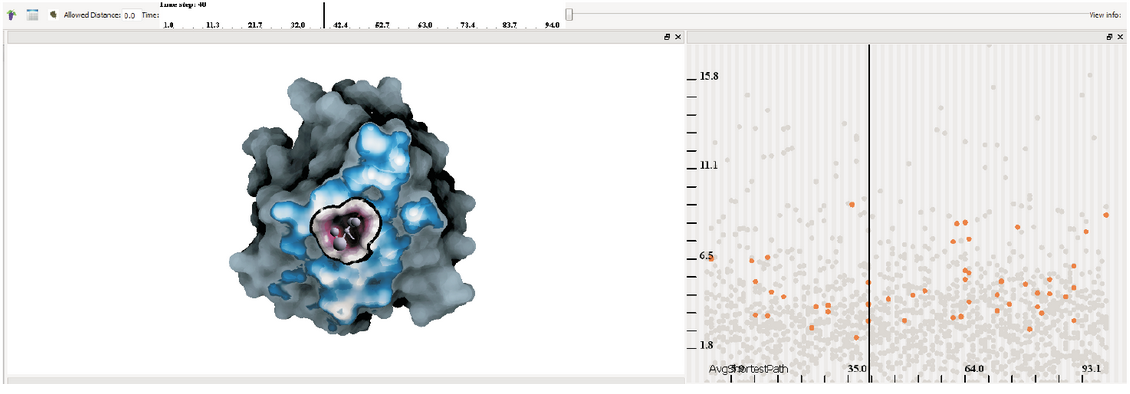
\includegraphics[width=0.7\textwidth]{pics/parulek2.png}
\vspace{-5mm}
\caption{Combination of a 3D view onto the structure containing a cavity with scatterplots \cite{parulek2012implicit}.}
\vspace{-3mm}
\label{parulek}
\end{figure}

\subsection{Our Own Previous Work and Competences}
\vspace{-4mm}
To reach the goals of this project, which focuses on the expressive visualizations of interactions between proteins and their comparison, their integration into the visual analysis tool, and the formalizing of visual analysis systems, we need to involve researchers with complementary expertise.
The project requires specialists in computational analysis and visualization, visual analysis, and functional proteomics.
Therefore our team has the following structure.

The project will be coordinated by Barbora Kozl\'{i}kov\'{a} from the Department of Computer Graphics and Design (DCGD) at the Masaryk University.
Her research group is already actively cooperating with other project partners. 
The DCGD group has several years of experiences with research focusing on in-silico protein analysis and visualization.
In cooperation with biochemists from the Loschmidt Laboratories at the Masaryk University, they have developed the CAVER 3.0~\cite{caver} tool for the computation of tunnels, channels, and pores inside protein structures. 
This tool was positively and widely accepted by the target community which is confirmed by many citations of the corresponding publication~\cite{caver} (139 in WoS, to date 25-02-2016).
Along with the computational tool, the DCGD team also developed the CAVER Analyst visualization tool \cite{analyst} that enables the analytical visualization of detected pathways and their further evaluation through various statistical and abstracted representations. 
Here Kozl\'{i}kov\'{a} played a key role in the design of the tool and currently is the leader of the research group of CAVER Analyst. 
The tool integrates algorithms for fast rendering of molecular structures as well as their tunnels, both for static snapshots as well as for molecular dynamics simulations. 
The tool is multiplatform and is freely available to the community.
The download package and the installation instructions are available from the software webpage (http://www.caver.cz). 

The second partner, i.e., researchers from the SPEC group at the Masaryk University led by Jan Pale\v{c}ek, has a long term experience in studying protein complexes (see Pale\v{c}ek's CV). 
Their efforts are oriented towards SMC complexes \cite{guerineau,hudson,Palecek2015}.
The DCGD and SPEC groups already established a fruitful mutual cooperation in the field of protein-protein interactions which is realized via an internal grant of the Masaryk University, started in 2016.
The cooperation involves also PhD students performing a thorough study of existing approaches for protein-protein docking.
Both research groups are affiliated with the same university so personal meetings are already happening and are easily organized on a regular basis.
 
On the Austrian side, the project will be led by Ivan Viola, from the Institute of Computer Graphics and Algorithms (ICGA) at the TU Wien. 
Viola worked on the acceleration of rendering of very large molecular systems~\cite{lampe} based on geometry shaders. 
Later on, the group has focused on novel geometric representations using implicit surfaces~\cite{ParulekViola2012}, which is an enabling technology for the interactive visual analysis of surface cavities~\cite{parulek2012implicit,parulek13visualanalysis}. 
The group also focused on an implicit hierarchical representation of molecules for the purpose of a seamless level of detail transition \cite{parulek13seamless}.
The latest publications focus on the illustrative visualization of large molecular systems and the visual guidance concerning ongoing reactions in these systems \cite{Muzic2014}.
The group also recently published the cellVIEW tool~\cite{cellview} focusing on illustrative and multi-scale rendering  of large biomolecular datasets. 
Large molecular systems were also studied with respect to attention guidance in dynamic narrative visualizations \cite{waldner}. 
In cooperation with the University of Bergen, they presented a method for interactively illustrating polymerization using a three-level model fusion \cite{kolesar} which depicts physiological polymerization processes at different time scales.
 
Between October 2014 and March 2015, Barbora Kozl\'{i}kov\'{a} was a member of the team of Prof. Viola at ICGA during a research stay, establishing a close cooperation in molecular visualization. 
The success of this effort is already evidenced by four joint papers. 
The first paper is related to the abstracted representation of temporal changes in a protein tunnel bottleneck (narrowest site) and its surroundings~\cite{molecollar}. 
It was presented at the EuroVis 2015 conference and also published in the Computer Graphics Forum journal~\footnote{https://www.eg.org/index.php/publications/computer-graphics-forum}. 
The second paper again focused on protein tunnels and their temporal evolution~\cite{animoamino}.
This time the study concentrated on the whole tunnel along its centerline, changes of the tunnel shape, and exploration of the surrounding amino acids with respect to their properties and extent of influence of the tunnel.
This paper was presented at the IEEE VIS 2015 conference and was published in the IEEE TVCG (Transactions on Visualization and Computer Graphics) journal~\footnote{http://ieeexplore.ieee.org/xpl/RecentIssue.jsp?punumber=2945}.
The third paper was a state-of-the-art report on molecular visualization where nine authors from several institutions joined their efforts~\cite{kozlikova_visualization_2015}. 
This report has been coordinated by Dr. Kozl\'{i}kov\'{a} and was accepted and presented at the EuroVis 2015 conference. The report was also invited for publication in the Computer Graphics Forum journal.
The report was followed by a survey accepted to the EuroVis 2016 conference. 
It focuses on the analysis and visualization of molecular cavities.

The DCGD and ICGA groups were also successful in obtaining a mutual mobility project (the OeAD ICM through project CZ 17/2015) for 2015 and 2016.


%%%%%%%%%%%%%%%%%%%%%%%%%%%%%%%%%%%%%%%%%%%%%%%%%%%%%%%%%%
% Section: Technical Description ---------------------------------------------
\section{Technical Description}
\label{sec:TechnicalDescription}
\vspace{-4mm}
The project is driven by the needs of the functional proteomics research, which to date does not take advantage of effective analytical workflows based on visualization.
It is unclear how to extend existing molecular visualization approaches reviewed in the previous section that would lead to a satisfactory solution of the yet untackled protein-protein interaction problem.
In our proposed solutions, we will start out from relevant real-world problems the researchers are facing when exploring and comparing different conformations of interacting proteins.
In tight cooperation between the project partners, these problems will be systematized into a set of tasks. 
The proposed visual representations will then be designed to fulfill these tasks.
Such tasks can be, e.g., T1: explore all possible conformations and easily filter out those conformations which are probably biochemically irrelevant, T2: briefly explore the individual conformations and their pairs of amino acids to support the decision process of task T1, T3: explore and compare the 3D shape of several conformations, along with the position of their contact zones, T4: explore the shape of the contact zones, T5: explore individual amino acids in the contact zones, their interaction and physico-chemical properties, T6: explore all possible conformations for multidocking, etc.

In the following sections we present two main stages of the project in detail. These stages are:
\begin{itemize}
\item Defining and systematizing the set of tasks and proposing novel visualization techniques enabling to fulfill these tasks. It will be followed by the design of an interactive visual analysis environment which integrates the selected proposed visualizations into one compact tool serving mainly for fast and intuitive exploration of the contact zones between proteins. %The complexity of the proposed environment will be reduced by tracking the interaction history with individual views of the visual analysis system.
%For example, the proposed visualization will enable to explore and compare different solutions for protein-protein interactions. These will be based on 3D views (e.g., exploded views) as well as on semantically driven 2D abstractions.
\item Proposing a formalism of visual analysis systems dealing with multi-faceted computational biology data and complex tasks. Such a formalism will categorize the individual visualizations according to the tasks they are able to support. Then it will enable to automatically suggest a set of the most suitable visualizations according to a given set of tasks defined within the first stage and these visualizations will be combined into a visual analysis coordinated multiple-views framework.
\end{itemize}

The algorithms suggested on the basis of the below delineated research ideas will be validated by a prototypical implementation in the CAVER Analyst visualization framework. 
Their potential utility factor will be evaluated in the context of the proteomics domain problem. 

%%%%%%%%%%%%%%%%%%%%%%%%%%%%%%%%%%%%%%%%%%%%%%%

\subsection{Stage 1: Comparative Visualization of Docking Ensembles}
\vspace{-4mm}
One of the biochemist's task is to select the most appropriate conformation for a particular pair of proteins.
Typically a set of automated computational procedures is launched (see Section \ref{sec:StateOfTheArt}), resulting in an ensemble of potential contact zones.
%The other possible scenario for the use of the newly proposed visualization methods is to employ the existing information about known interactions between proteins (taken, e.g., from the PDBsum database).
This information can be used as a reference when searching for the unknown contact between similar proteins (e.g., from the same family of proteins). 
A promising strategy is to combine these two approaches and, if possible, use the database entries to find the most biochemically relevant solutions in the ensemble calculated with a computational tool, such as HADDOCK~\cite{haddock} or PyDOCK~\cite{pydock}.

For this purpose, we plan to design several visual representations which will convey different types of information about the interacting proteins.
On the highest level, the users should have an overview of all conformations which should be explored. 
For this purpose, we suggest an abstracted interactive representation which enables the user to see the overall potential interaction pattern and to filter out conformations not fulfilling a given set of criteria (task T1).
As an example, one such criterion could be that one pair of interacting amino acids is assumed to contribute to the interaction. 
Such a hypothesis is often formed by the biologists in the early stage of the analytical workflow. 
Such a representation will combine a \textbf{matrix-based visualization} with additional views highlighting the interacting amino acids in a selected conformation (task T2).
Figure~\ref{fig:matrix} illustrates these ideas. 
Rows and columns of the matrix correspond to all amino acids in the contact zones of the interacting proteins. 
The cells are colored according to the frequency of occurrence of the given pair of amino acids in the conformations -- the more red color, the more often the pair in the set of all conformations is present.
The column on the right side of the matrix will enable to explore one of the conformations (centered to be in focus) and its interacting pairs of amino acids (highlighted by the red line).
%It consists of the matrix view and an interactive lens view where each rectangle corresponds to one conformation and for the conformation in the focus (center) the corresponding pairs of amino acids are connected.

\setlength\intextsep{0pt}
\begin{wrapfigure}{r}{0.7\textwidth}
\vspace{-3mm}
  \begin{center}
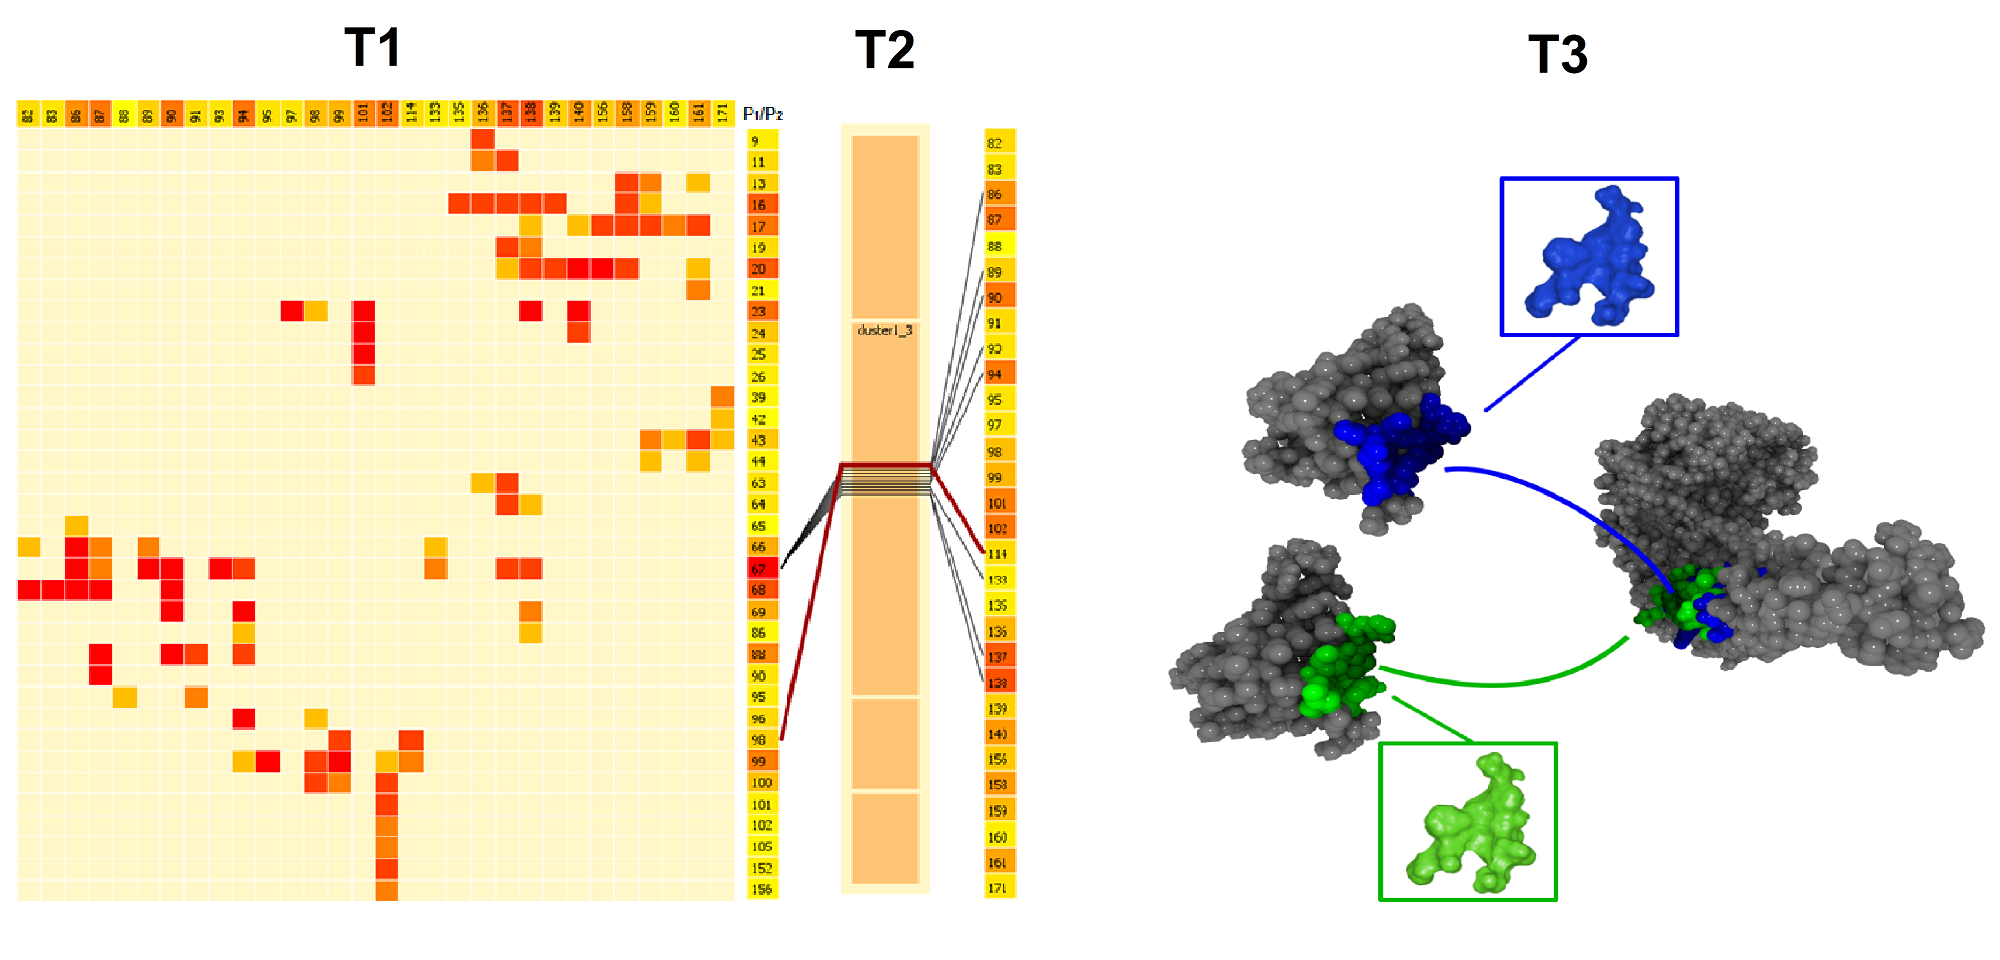
\includegraphics[width=0.7\textwidth]{pics/matrix2.png}
\end{center}
\vspace{-5mm}
\caption{T1: matrix view showing an overview of all conformations. T2: lens view highlighting individual pairs of amino acids for the conformation in focus, T3: 3D exploded view enabling to show several conformations at once and to highlight the contact zones.}
\label{fig:matrix}
\end{wrapfigure}

The exploration of molecules in 3D space reveals structural properties to the biochemists.
However, as already shown directly in Figure~\ref{fig:problem}, simple superposition is not an acceptable solution as this leads to severe clutter and does not scale well with the number of conformations.
Contact zones are very important but easily affected by occlusion problems.
Therefore we propose to adapt the technique of \textbf{exploded views} (see Figure~\ref{fig:matrix}) which will be equipped with a closeup view (task T3).
In these closeups, positioned close to the translated (exploded) protein, we will be able to present additional information about the contact zones (tasks T4 and T5).

In the closeup view we propose to present a trimmed \textbf{semi-flattened view} of the contact zone (positioned perpendicularly to the user; Fig.~\ref{fig:preview}a), the \textbf{neighborhood map} of individual amino acids in the contact zone (Fig.~\ref{fig:preview}b), and the mutual distances between the interacting amino acids using a \textbf{height map} (Fig.~\ref{fig:preview}c).
We propose to embed a simplified contact zone representation into a comprehensive 3D context with the addition of supporting guiding lines.
For individual conformations, these maps can be also visualized as illustrated in Figure~\ref{fig:preview}d.

The occlusion problem is caused by the fact that often the computational tools output candidate interaction conformations that are very similar to each other and differ only by a small shift on the surface or a small rotation angle.
To tackle this we plan to use aggregated visual representations which will find the best representative of a set of aligned reference proteins which are very similar with respect to their spatial orientation (see the set of aligned reference proteins in green in Figure~\ref{fig:problem}).
The representative can be selected, e.g.,  as the median, average, or the most central from all the representations of the reference protein.
For distributions of a single random variable, box plots are already widely used (and already extended to curves).
However, we have to extend these concepts to complex geometric structures like molecular conformations, ensembles of molecular surfaces, and ensembles of secondary structures.

Another possible solution will be the usage of reformations when we translate the problem to lower-dimensional representations which are simpler than the original 3D situation and which allow the user a standardized comparison. 
In the context of protein-protein interactions, this means, e.g., to display the contact zones directly on the molecular surface of the interacting proteins, flatten these surfaces and show many contact zones as overlapping contours in this simplified representation.
As the data has to be viewed with different levels of detail, we will introduce domain-semantic based "levels-of-complexity". 
This will enable the user to explore, e.g, a contact zone, on different levels of abstraction or detail.
To give an example, the contact zone can be viewed just as an entry in the list of all possible contact zones, it can be visualized as a surface in 3D, a 3D surface with indicated interacting amino acids, 3D surface with indicated properties of these amino acids, a 2D-flattened polygon, etc.

%\setlength\intextsep{0pt}
\begin{figure}[ht]
%\vspace{-5mm}
\centering
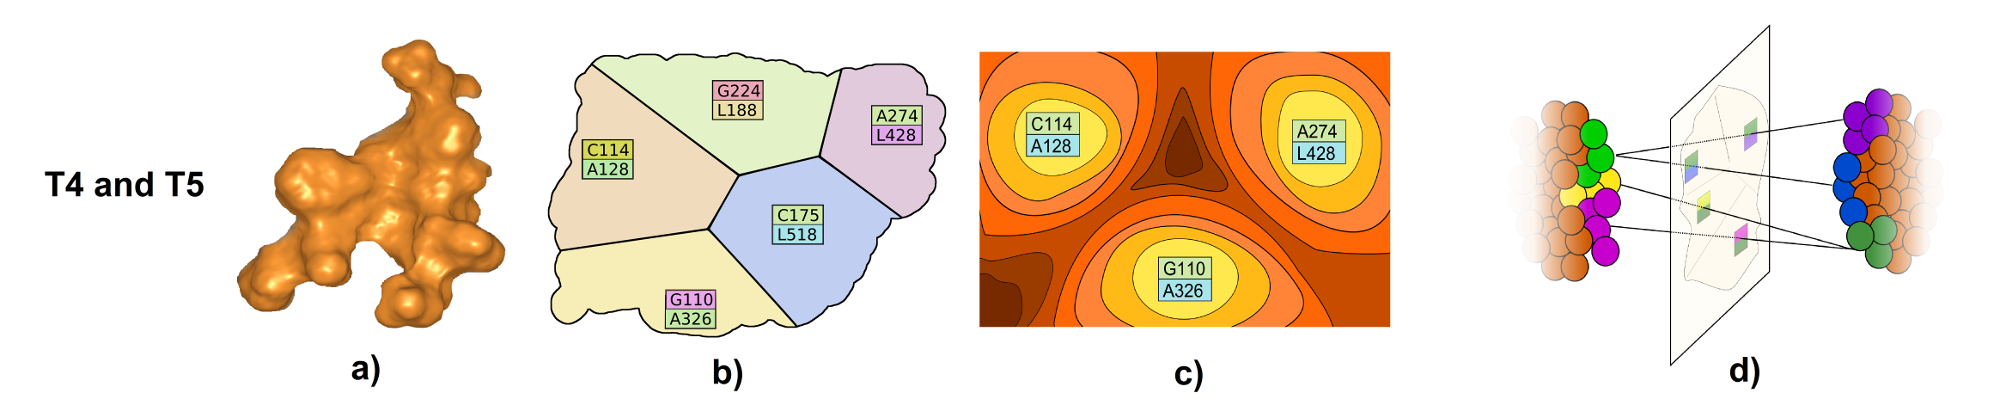
\includegraphics[width=0.9\textwidth]{pics/previewsmall.png}
\vspace{-3mm}
\caption{a) View on the contact zone (should be semi-flattened). b) Neighborhood map of individual amino acids in the contact zone. c) Height map showing the mutual distances between amino acids in the contact zone. d) For individual conformations, the preview can be positioned between the interacting proteins.}
\label{fig:preview}
\end{figure}

\subsubsection{Visualizing Multidocking Search-Space}
\vspace{-3mm}
Initially, we will use available docking computations to generate ensembles of pair-wise dockings among all involved proteins forming the complex. 
Some contact zone candidates will naturally conflict with each other by competing for the same surface area. 
We will investigate visualization metaphors such as a pairwise multidocking matrix (see Figure~\ref{fig:multidock2}), where the analyst can choose a particular contact among two proteins (task T6). 
Instead of using one matrix as in the previous case, now for each protein interaction there is a separate matrix and they are concatenated together by the sequence of amino acids of one particular shared protein. 

Attention will be guided to contact zones with other proteins from the same complex, which are affected by \emph{occupying} the surface area by selected interaction. As the interacting proteins form complexes consisting of more than two proteins (results of multidocking), the corresponding visual representations will also face this increased clutter and occlusion challenge. It is an open question how to tackle it and whether or not exploded views are still a meaningful metaphor for conveying structural properties of the interaction.

Multidocking establishes a relationship between several molecules that form the molecular complex. In this sense, the relationship in the contact zone set is no longer binary, but $n>2$-nary, and an edge becomes a hyperedge in a hypergraph. 
We envision a contact-zone hypergraph to depict all possible relationships in the molecular complex. 
A hyperlink will essentially define one possible multidocking complex. 
From such a visual representation, we can see all possible contact scenarios, which contact zones are central, and we can rank these according to the overall or minimal stability.

We will experiment with taking the hypergraph as a basis for a heterogeneous visualization and will augment it with structural details.
Even if these will be severely distorted, the visualization will still communicate important geometric, physical, and chemical properties. 
This way, we will experiment with heterogeneous visualizations where the underlying relationships serve as the basis, and the structure augments further aspects on top of the basis.


%\begin{figure}[bh]
%\centering
%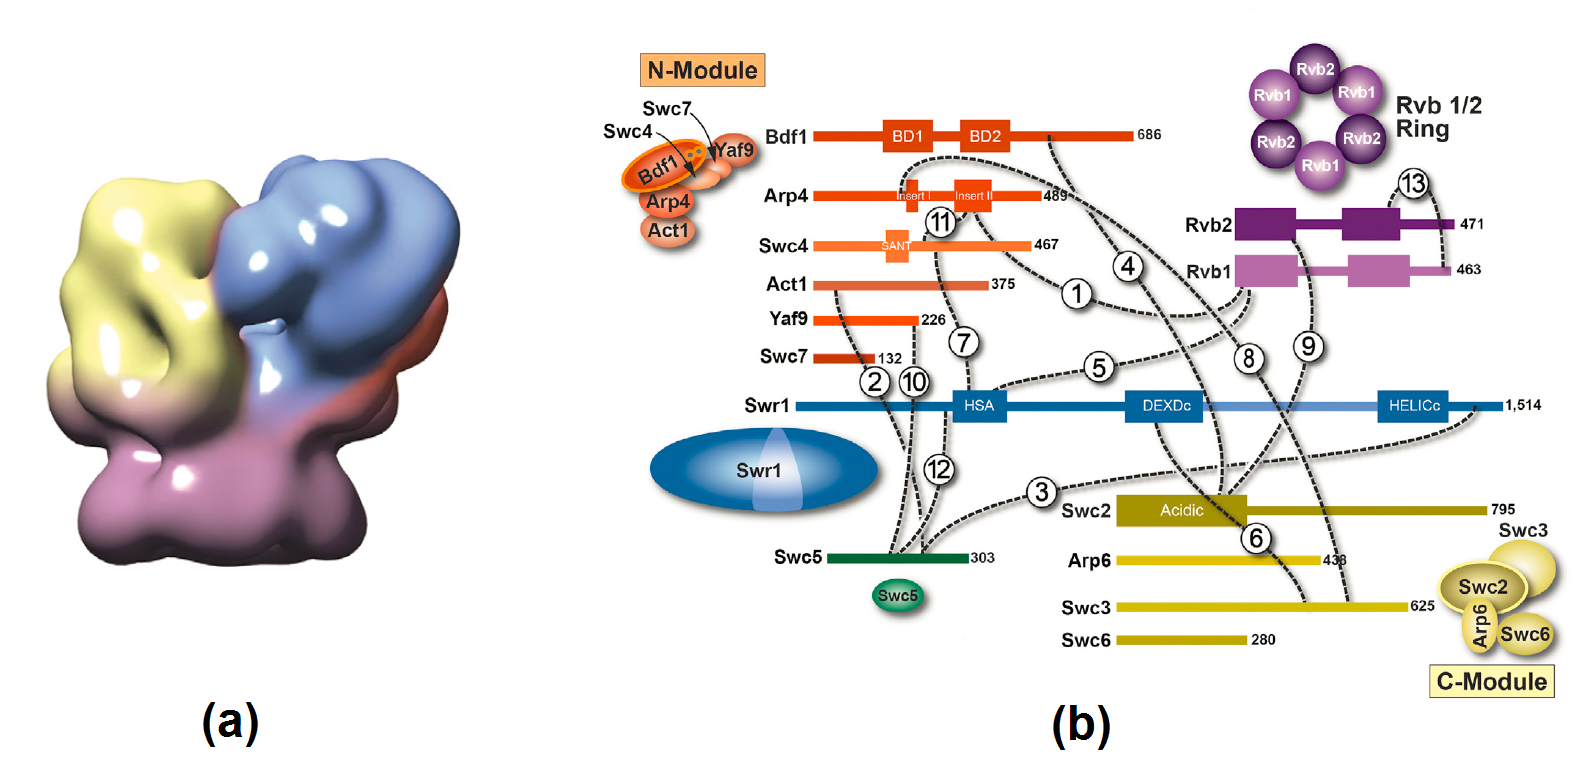
\includegraphics[width=0.6\textwidth]{pics/multidock.png}
%\caption{(a) 3D representation of the protein complex, (b) schematic representation of interprotein crosslinks in the complex consisting of 14 proteins \cite{Nguyen}.}
%\label{fig:multidocking}
%\end{figure}

\setlength\intextsep{0pt}
\begin{wrapfigure}{r}{0.4\textwidth}
\vspace{-5mm}
  \begin{center}
    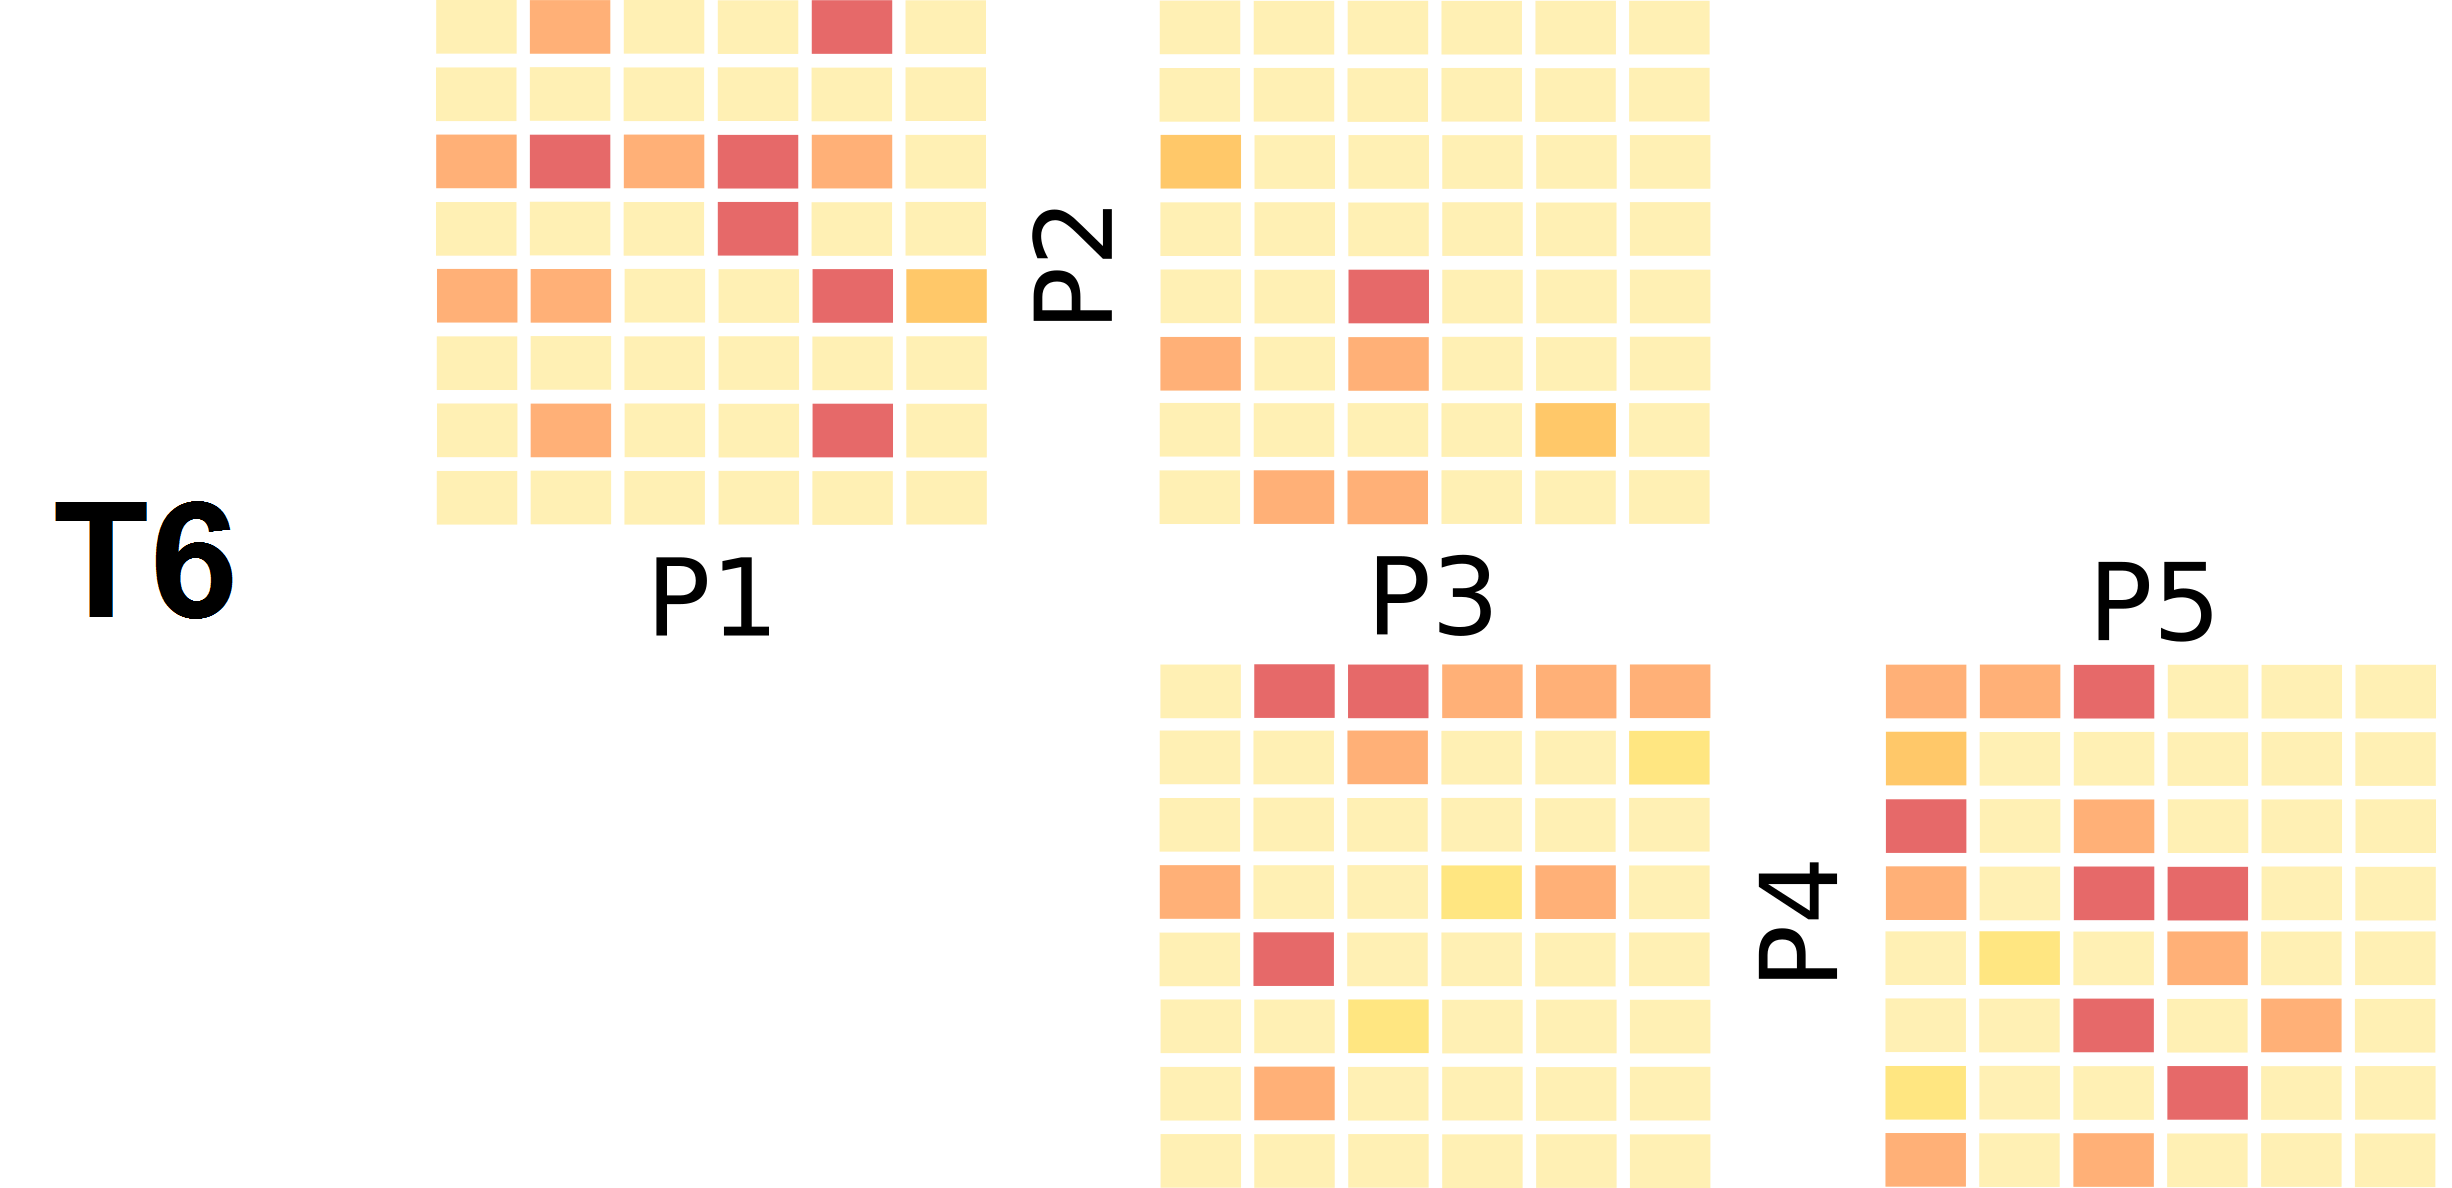
\includegraphics[width=0.4\textwidth]{pics/multidock2.png}
  \end{center}
\vspace{-5mm}
  \caption{Interactive multidocking matrix enabling to show the overview of all conformations between proteins P1 -- P5. P1 interacts with P2 which also interacts with P3, etc.}
  \label{fig:multidock2}
\end{wrapfigure}

During the analysis, the history of contact-zone evaluation will be provided so that the analyst avoids reevaluating already assessed surfaces. 
Visual guidance has the potential to improve this analytical stage substantially, as minimal-conflict high-probability contact complexes can be suggested to the analyst for a prioritized assessment over scenarios that are far less likely to form a molecular complex.

After a particular selection of a preferred multidocking scenario, MD simulations will further assess the stability of the given setup. 
Should the tested complex scenario turn out to be unstable, this information is then propagated back into the contact-zone hypergraph representation, so that other constellations will be prioritized in ranking and consequent visual analysis.

\subsubsection{Comparison of Conformations from Different Computational Tools}
\vspace{-3mm}
If the source of the input data is made-up by the results of various computational tools, it is not advisable to simply combine them into one common input.
The main reason is that these tools produce slightly different output parameters (e.g., each tool computes its own scores). 
Therefore, the proposed visualizations should need to be extended. 
For example, each cell in the matrix visualization illustrated in Figure~\ref{fig:matrix} will be divided according to the number of used computational tools and each part will correspond to one tool.
Visual reduction operations based on semantic domain knowledge will reduce visual complexity in the context region.
Such operations could be: take the worst/best solution, just highlight high-variance regions, indicate biased areas, etc.


%%%%%%%%%%%%%%%%%%%%%%%%%%%%%%%%%%%%%%%%%%%%%%%%%%%%%%%%%%%%%%%%%%%%%%%%%

\subsubsection{Visual Analysis of Interactions}
\vspace{-3mm}
Subsequently, we will propose several combinations of the designed visualization techniques into visual analysis tools aiming to provide the users with an intuitive and interactive environment supporting their tasks.
However, the input data as well as the tasks can be highly complex which will in consequence lead to too complex visual analysis tools containing too many linked views.
As a solution to this problem we will propose a semi-automatic simplification of such tools through adaptation.
It will be based on the tracking of user interaction with a given tool when performing a specific task.
Based on the interaction history with individual views (i.e., how often the view was used by the user) we will decide which views should be removed or replaced by other ones. 
This user-centered approach to the design of the visual analysis tool tailored to a specific set of tasks will enable to utilize such a tool very effectively.

%According to the set of the tasks defined by the domain experts, we will propose the set-up of the resulting tool.
All visualizations used in the tool will be interlinked and by using advanced brushing methods the tool will serve exploration, comparison, simplification, and other required functionality.
%The visual analysis tool will support customization so the users will be able to further adjust the set of the integrated visualizations to fulfill a given task.



\subsection{Stage 2: Formalization of Visual Analysis Systems}
\vspace{-4mm}
If we look back in the visual analytics (VA) research in the past decade, there have been many VA frameworks proposed, which aid the completion of a particular visualization task. Many of them appear to have a similar high-level pattern, the mostly utilized pattern is the juxtaposition of different views which reveal one or few aspects of a multi-dimensional phenomenon. A VA framework typically provides views for each aspect that is necessary to understand to accomplish a given analytical task. These aspects are linked together so that their mutual relationships can be understood as well. These are the famous multiple coordinated views.
In such a visual analysis framework, sharing of variables across views is important.
An interesting aspect here is the placement of the views so that the most related information is close on the display. 

Our task analysis, of which preliminary results are listed in the previous section, offers several scenarios for which a tailor-made VA framework can be designed. Until now, this has been done by visualization experts themselves. However, in case we have a clear structure about the aspects which describe a given phenomenon and at the same time we have clearly defined tasks, we hypothesize that it should be possible to design the VA framework algorithmically. In the second stage of the proposed research we will focus on developing a formalism for a VA design and contribute to the theoretical foundations to this emerging subfield of visualization. 

To propose a formal systematization for such structured data, the overall goal is to enable a systematic exploration of the underlying design space of possible visual representations and interactions.
Until now, when designing visualizations for a specific target domain, the typical procedure is to perform an analysis of requirements and according to them design the most suitable visualizations for the whole visual analysis system. 
However, this obviously leads to a constantly repeating process (even for slight task changes) which is based on the same principles and mostly ad-hoc approaches have been used to propose a specific visual representation for a specific task situation at hand.
Therefore, a drill down into relevant subparts of the highly structured data must be done with typical database queries but with a strong domain semantic from our application area. 
Operations used for the extraction of these subparts could be, e.g., slicing, dicing, projections, aggregations, etc. 
For each of these operations the appropriate visual templates need to be developed.

The selection of relevant subparts will be driven by the user-defined tasks.
These tasks are likewise highly complex and are usually formed by the combination of much simpler basic tasks, such as T1, ..., T6 mentioned in the Stage 1 of the proposal. 
As the set of basic tasks can be large and combining them creates a vast space of possible queries, we need a systematic formalization here as well.
In order to propose the formal system based on different user tasks, the definition of these tasks has to be structured as well. We will base our considerations on the recent task taxonomies in the visualization research literature. 

Instead of defining the VA design explicitly, the specification will be of a declarative nature so that even a domain specialist would be able to implicitly author the VA framework.
For specification we will create a domain-specific language for the definition of these tasks which will serve as a meta-language for the automatic selection of relevant visualizations and their integration into the overall visual analysis system. The syntax of the language will combine traditional commands of programming languages with naming conventions of the given domain. The functions derived from a set of basic as well as complex tasks will form the basis of the semantic meaning of the language. Here we will be inspired by a feature definition language proposed by Doleisch et al.~\cite{Doleisch} who presented a framework for flexible and interactive specification of high-dimensional and complex features in simulation data. It allows the definition of one or several features by brushing multiple dimensions and highlighting the selected features in all linked views.
In our case, such features of the input data are, e.g., two interacting proteins, a set of interacting proteins (larger than two), contact zones, interacting amino acids, temporal changes of the proteins, etc. 
As the tasks will change, because of progressing in the analytical workflow, we will also investigate how to smoothly adapt the interface so that the change between the layout for the previous and current task is continuous instead of building entirely new graphical user interface.

A naive approach to build a VA workflow would be to include all possible visualizations from the predefined set to show all possible kinds of relationships. If the display estate is huge, such approach is possible to implement. However, this would result in too much of visual information to be effectively consumable during the analysis workflow. Humans have only a limited field of view, they could be easily overwhelmed, so the display space needs to be utilized that only most crucial visualization views are included in the VA framework design. The VA design would then be constrained from both sides, the necessity to show particular visual information and the availability of visual estate. We will investigate whether force-based approaches would be suitable for resolving the constraints. At the first glance procedural modeling of architecture might sound like not very relevant for automated design of VA frameworks. Especially the recent works on interior design or scaffold structure deal with a similar problem. On one hand there is the desired functionality, on the other hand there are technical norms and space limitations that constraint the design choice. While it is at this moment rather open what is a feasible solution for automated VA design, we will seek for inspiration in related visual computing domains to tackle such high-risk high-gain research objective.



%Moreover, when dealing with large-input, heterogeneous data and complex tasks, the design process usually covers only a small subset of possible tasks.  
%If the input data is highly structured, such as in our case of protein-protein interactions, we can propose visualizations focusing on different aspects of the input dataset.
%Therefore, in close cooperation with the domain experts, we will define a systematic description of individual characteristics playing an important role in the exploration of protein-protein interactions.
%Based on this information, we will propose a formalized model which will categorize the suggested visualizations into clusters according to these characteristics and their basic properties (examples in Figure~\ref{fig:system}, Stage 3).
%Then for a given task, we will automatically suggest the combination of clusters which will form the resulting visual analysis system presented to the user. 
%In consequence, different tasks can lead to different visual analysis systems.


\subsection{Integration of Visualization Technologies}
\vspace{-4mm}
The visualization research described in the previous sections is motivated by the needs of analyzing data in proteomics and structural biology. 
The ambition is to utilize these technologies in new analytical workflows.
We will therefore build a meaningful selection of the proposed approaches into one software framework, integrated into the CAVER Analyst visualization software. 
As a part of this system integration, we plan to perform studies on the usability of the entire system, and we will employ iterative design strategies for making the system intuitive to use by the experts. 
This will be primarily done during the technological development. 
In relation to the validation part of the proposed research described below, where the system will be employed in an actual scientific workflow, we will assess the system's accuracy and stability with respect to the experimental data provided by the domain experts.


\subsection{Usability Testing in Proteomics Research}
\vspace{-4mm}
\label{sec:smc}
The goal of this research focus is to apply and test the above visualization technologies on real SMC complexes. 
The SMC complexes have a unique architecture suited for their role as chromatin organizers~\cite{Palecek2015}. 
The SMC subunits form rings (see Figure~\ref{fig:telomere}) which can be temporarily opened to load or release chromatin fibre~\cite{Haering2016}. 
Specific bindings of non-SMC (NSE) subunits at one end of the SMC ring regulates its closure. 
Mapping of these interactions provides the information about the positioning of the NSE subunits and may suggest loading/exit paths for DNA fibres.

The new software framework developed within this project will enable us to compose and visualize a complete hypothetical SMC complex with its dynamics. 
Such an insight will help us to advance the understanding of the SMC architecture and its dynamics.
 
In this validation stage of the project, we will analyze all the available ($>$10 PDB) crystal structures of prokaryotic and eukaryotic SMC complexes~\cite{Palecek2015}. 
We will model protein structures of their homologs (e.g., yeast proteins will be modeled based on bacterial and human crystal structures), combine partial information from these different structures and make a general model of a complete SMC complex. 
Similarly, other complexes studied at the group of DFGP (e.g., telomere-associated shelterin complex~\cite{Janouskova2015,Schrumpfova}) will be analyzed and presented within the semestral course of "Protein complexes" (taught by Dr. Pale\v{c}ek).




%\section{Project Plan}

\section{Project Management}
\vspace{-5mm}
The project management can be divided into research activities and project administration.
The research activities will be coordinated by Barbora Kozl\'{i}kov\'{a} and Ivan Viola. 
They will be responsible for the scientific results and progress of the project.
The administration of the project will be managed by Barbora Kozl\'{i}kov\'{a} and Ivan Viola, the representatives of the project on the Czech and Austrian side, respectively. 
Dr. Kozl\'{i}kov\'{a} and Prof. Viola will be responsible for the scientific and financial reports, which will be prepared jointly by both partners and their financial administrators. 

The coordination of both partners will be carried out by frequent meetings. 
Because of the geographical distribution and interdisciplinarity of the project, special coordination and communication strategies are necessary. 
This includes a database for storing joint literature and publications and repositories for easy software deployment. 
The shared database and repositories will be maintained using the graphical workstation required for this project. 
Moreover, we will organize regular project meetings (four meetings of the whole project team per year) and yearly workshops, where our latest results will be presented to colleagues and students at the corresponding departments. 
We will also establish a collaboration on an institutional level, where we will arrange several reciprocal internships of young researchers (via mobility projects or the ERASMUS+ study program). The initial project meeting will be organized in January 2017 in Brno, the project end meeting will be held in Vienna. 
Regular meetings will be held in Vienna, in Brno or half way between these two cities, in Mikulov.


% Section: Timetable -----------------------------------------
\section{Timetable}
\label{sec:Timetable}
\vspace{-5mm}
The project timetable, illustrated in Figure \ref{timetable}, details the time spread of the individual stages along with the integration and evaluation steps.
\vspace{3mm}
 
%\setlength\intextsep{0pt}
\begin{figure}[h]
\centering
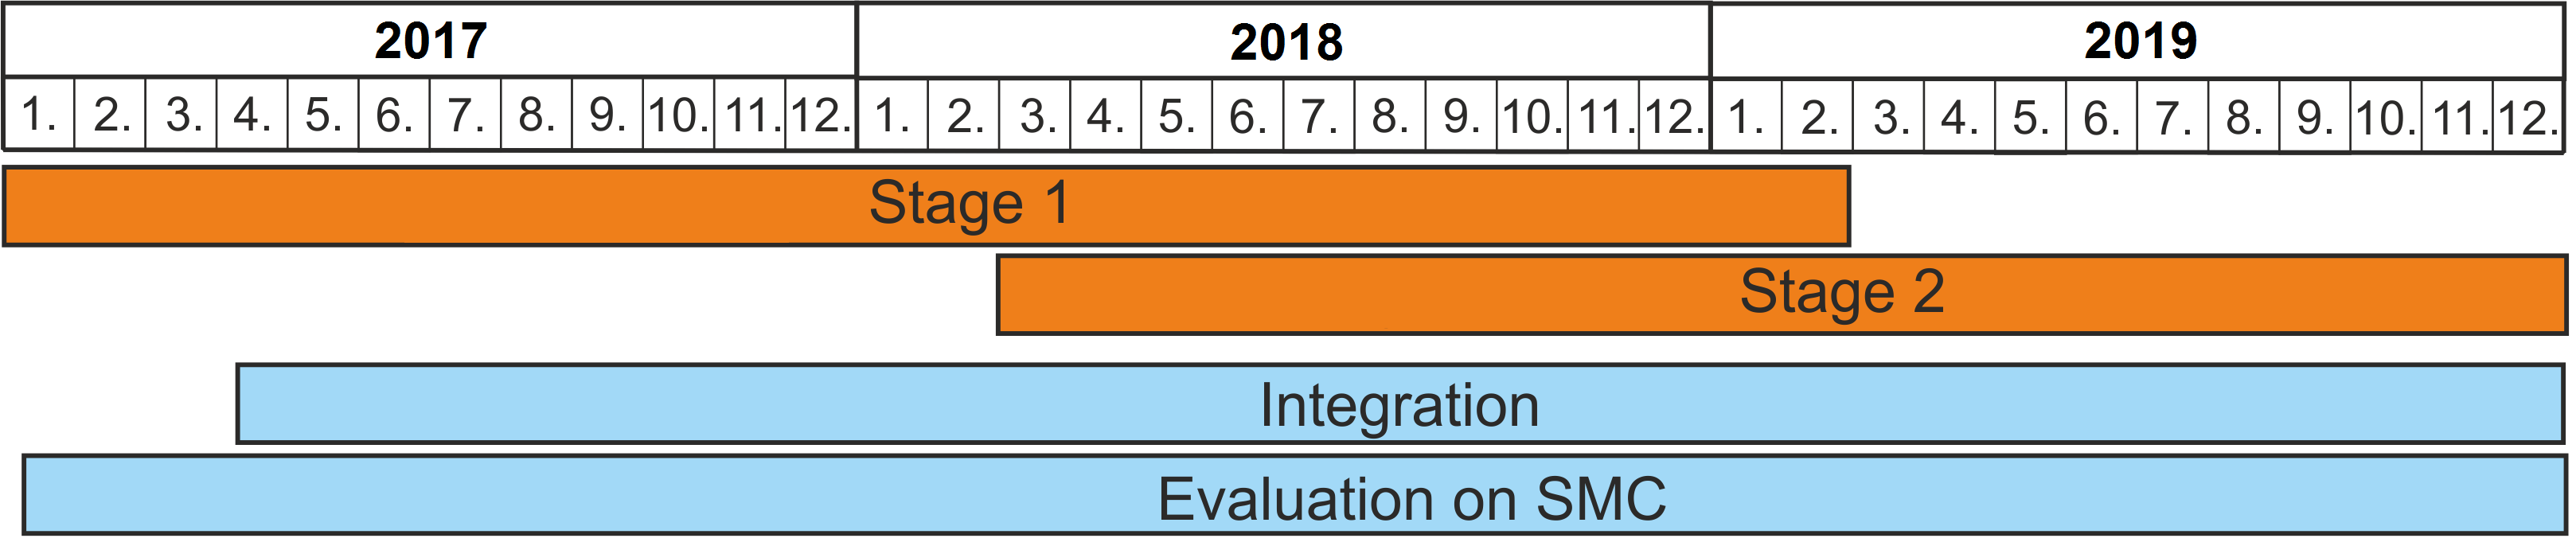
\includegraphics[width=0.8\textwidth]{pics/timeline.png}
\caption{The proposed timetable.}
\label{timetable}
\end{figure}

Stage 1 will be coordinated by Dr. Kozl\'{i}kov\'{a}. 
In this stage, a very tight cooperation with experts from SPEC will be crucial, so the personal meetings between members of DCGD and SPEC will be held on a regular (weekly) basis. 
The design of the novel methods will gain from the experience of the ICGA group, and the preliminary results will be immediately tested and evaluated by the SPEC group. 
Stage 2 will be coordinated by Prof. Viola and along with Dr. Kozl\'{i}kov\'{a} and their teams they will cooperate on the design of the proposed formal system. 
The design of the system will highly depend on the user requirements which will come from Dr. Pale\v{c}ek who will be also responsible for coordinating the evaluation and testing phase.

All proposed methods will be integrated into one software framework, CAVER Analyst. This activity will be coordinated and mostly implemented by Dr. Kozl\'{i}kov\'{a} as her research group is the author of this software tool. The methods will be intensively tested on the SMC complexes and this testing will take place throughout the entire project.

\subsection{Dissemination Plan}
\vspace{-4mm}
This basic research project on visualization will be published first in primary scientific venues for visualization research. These include IEEE TVCG (IEEE VIS Conference) and EG CGF (EG EuroVis Conference). Focused events on visualization of biological data, such as IEEE BioVis (in particular in connection with BMC Bioinformatics) or EG VCBM will be also considered for publication of the project's results. We expect approximately 8-10 visualization papers published in primary venues on visualization.

The integration into a system for visualization and analysis of protein-protein interactions will be published in a bioinformatics journal. Currently we have BMC Bioinformatics in mind. In case the new workflow enables a major scientific breakthrough, we will prepare a Nature Methods paper. 

%The project web page will be established at the beginning of the project and will contain the basic information about the aim of the project, the research team and the core activities. The content will be systematically updated according to the project progress. The link to the project web page will be also included into the existing group web pages on both institutions.

%Moreover, the project will be promoted at the publicly available annual Researchers' Night event, at which the Masaryk University actively participates. 
New tools will be presented to regular master students subscribed to the “Proteomics” course and the course on “Structure and function of protein complexes” taught by Dr. Palecek. For presentation and educational purposes, we also aim to print the sub-complexes in a selected spatial conformation on a 3D printer. 

\subsection{Risk Analysis}
\vspace{-4mm}
Risks with respect to the quality and usability of project outputs are related to the performance of the created framework,  individual proposed methods, and the accuracy and scalability of the developed methods. Other risks are: the graphical user interface (GUI) of the framework will not be accepted by domain experts, some of the proposed visualization methods will suffer from visual clutter, the proposed interaction techniques will be too complex, there will be still unknown limitations in the target domain preventing to create a sufficient formal system.
To avoid these problems, we will profit from our previous experience in creating optimized accurate software tools \cite{caver}, as well as in designing domain specific visualization, GUI and interaction \cite{analyst}, and many years of expertise in the visualization and visual analysis domain (ICGA). 

Numerous structures of protein complexes are available in the PDBsum database, therefore, if the SMC complex focus fails we can refocus on to the other DFGP studied complexes or any PDBsum (chromatin-associated) complex familiar to Dr. Pale\v{c}ek. 
% Section: Research Institution -----------------------------------------------
\section{Research Institution}
\label{sec:ResearchInstitution}

\subsection{Location}
\vspace{-4mm}
On the Austrian side, the research will take place at the Computer Graphics Group of ICGA, Vienna University of Technology, which performs extensive fundamental and applied research in computer graphics and visualization. 
Its areas of expertise are modeling and rendering, scientific visualization, virtual environments, and computer animation. In the field of scientific visualization the research is focused on advancing medical visualization, in particular medical ultrasound, illustrative visualization, knowledge-assisted visualization, visual analysis of parameter spaces, and point-based visualization. The Visualization Group at ICGA has also developed and implemented an open-source visualization prototyping environment, i.e., VolumeShop. In the area of scientific visualization there are long standing cooperations with the Austrian Academy of Sciences, the General Hospital in Vienna, VRVis, Austria; University of California, Stanford University, USA; University of T\"{u}bingen, University of Stuttgart, University of Rostock, University of Magdeburg, Germany; INRIA Research Institute, University Joseph Fourier, France;  University of Girona, Spain; TU Budapest, Hungary; CTU Prague, Masaryk University in Brno, Czech Republic; Comenius University in Bratislava, Slovakia; and University of Bergen, Norway.

The Czech part of the team consists of two departments at the Masaryk University in Brno.
The first research group comes from the Department of Computer Graphics and Design (DCGD) located at the Faculty of Informatics of the Masaryk University. 
The computer graphics group consists of two associate professors, two assistant professors and nine PhD students. 
The main research areas of the group are human-computer interfaces, virtual reality, haptic interfaces, computational geometry and visualization. 

The second group of researchers from the Masaryk University involved in this project is the SPEC group of Dr. Pale\v{c}ek. 
The main research areas of Pale\v{c}ek's group are architecture, structure, function, and evolution of protein complexes.
Its members focus on studying protein-protein and DNA-protein interactions using a wide range of biochemical approaches (e.g., yeast two-hybrid, pull-down, immunoprecipitation, peptide libraries, mutagenesis, etc.). 
In addition, the Pale\v{c}ek lab collaborates with NMR and cryoEM (CEITEC) and crystallographic groups (at Sussex University, United Kingdom). 

\subsection{Personnel}
\vspace{-4mm}
\textbf{Dr. Barbora Kozl\'{i}kov\'{a}}, the project coordinator, is an assistant professor at DCGD, Faculty of Informatics, Masaryk University in Brno. In 2011 she has received her PhD from the same university. She focuses mainly on the interdisciplinary CAVER project which integrates computational geometry and visualization. She is the co-leader of the Human-Computer Interaction Laboratory (www.decibel.fi.muni.cz). 

\textbf{Prof. Dr. Ivan Viola} is an assistant professor at ICGA, Vienna University of Technology (VUT) and adjunct professor at the University of Bergen, Norway. In 2005 he has received his PhD from VUT. In 2011, he received an WWTF Vienna Research Groups award which provides basic financing of his group for eight years. His research interests include computer graphics, visualization, with particular focus on illustrative visualization. He is co-heading the visualization group at ICGA. The group performs basic and applied research projects in the area of scientific visualization. 

\textbf{Assoc. Prof. Jan Pale\v{c}ek} is currently heading his own Structural Proteins of Eukaryotic Chromosomes group at  DFGP (Faculty of Science) at the Masaryk University. 
In addition, he is a senior researcher in Genomics and Proteomics of the Plant Systems program at CEITEC MU. 
He received his Dr.rer.nat. (equivalent to a PhD in biochemistry) from the Vienna University (Austria) in 1998 and habilitated (in molecular biology) at the Masaryk University (Czech Republic) in 2012. 
He is interested in protein-protein interactions and protein complexes. 
Since his postdoctoral stay at Sussex University (United Kingdom, from 2002 till 2006), he focuses on the architecture and evolution of the SMC and MAGE protein complexes. 
Dr. Pale\v{c}ek was awarded with a Czech Science Foundation (CSF) grant to study a "Role of non-SMC proteins in stabilization and processing of stalled replication forks" (GA13-00774S, 2013--2016).


\subsection{Available Equipment}
\vspace{-4mm}
\label{subsec:AvailableEquipment}
All participating institutes will provide the basic research infrastructure, including workplaces, basic hardware, licenses for operating systems and development tools, internet connection, and office supplies for their team members. 
Computation time on a grid architecture will be provided free of charge by the NGI Metacentre~\url{http://www.metacentrum.cz/} if needed. 

%The research environment of the Department of Functional Genomics and Proteomics at the Masaryk University provides technical infrastructure for all the lab work. 
%The laboratories are equipped for biochemical and molecular biology experiments (centrifuges and ultracentrifuges, UV/VIS spectrophotometers, FPLC chromatography, instruments for protein purification and analysis, cell cultivation facilities, cold rooms, deep freezers, autoclaves, incubators and shakers, PCR machines, radioisotope laboratory, documentation and detection systems for chemiluminescence and fluorescence). 
%In addition, the CEITEC MU institute (where Dr. Pale\v{c}ek is emplyed as senior research fellow) offers excellent state-of-the-art infrastructure (including cryoEM, NMR and crystallographic facilities, http://www.ceitec.eu/core-facility/list/).

% Section: Requested Funding --------------------------------------------------
\section{Requested Funding}
\vspace{-5mm}
\label{sec:RequestedFunding}

\paragraph{Personnel}
Apart from the applicants and the staff at the institutions who will participate in this research project, we request two full-time PhD positions, who will conduct the proposed research full time. 
One position will be covered by three part-time contracts for Katar\'{i}na Furmanov\'{a}, Adam Jur\v{c}\'{i}k and one of the new PhD student. 
They will be supervised by Dr. Barbora Kozl\'{i}kov\'{a}.
Additionally to this, Dr. Pale\v{c}ek will be 20\% engaged in the project.
%Based on our previous experience with similar research projects, we estimate that the time needed to achieve the goals of this project will require three years for the junior researcher position.
For the junior researcher at ICGA we plan to recruit a suitable candidate from new graduates of ICGA or graduates from other universities, who will meet the requirements.
This researcher will be supervised by Prof. Dr. Ivan Viola.\\
Total personnel costs AT = 109 980,00 EUR; total personnel costs CZ = 87 651,17 EUR\\
\textbf{Total personnel costs (including insurance):}   \textbf{197 631,17} EUR
\vspace{-5mm}
\paragraph{Equipment}
To efficiently conduct our research project we request one high-performance graphics workstation, software + updates (mainly graphics cards).\\
Workstation = 11 826,77 EUR 
\vspace{-5mm} 
\paragraph{Materials}
On the Czech side, the material costs will be used for high-performance graphics cards. As we plan to produce high-quality color posters to present our project at conferences and important local events, we involve these costs into the budget as well. Here we include also costs for organizing yearly project workshops with the participation of the involved researchers and participation of external experts.\\
Posters and 3D prints and workshops AT = 1 500,00 EUR; graphics cards, posters, 3D prints, workshops CZ = 5 991,35 EUR\\
\textbf{Total material costs:}   \textbf{7 491,34} EUR
\vspace{-5mm}
\paragraph{Travel}
The results of the project will be presented at international conferences, namely IEEE VIS, EG EuroVis, IEEE PacificVis. We expect to publish about 5 papers per year, (2 journal and 3 top conference papers), resulting in a total of 9 active participations of project members, 3 of which we expect to be in the US. For this we require 11,000 EUR in total (1,000 EUR per conference in Europe, 1,500 EUR per conference in the US).
The required traveling costs will also cover the expenses for meetings of project partners (3,000 EUR in total) and for research stays of PhD students participating on the project at the partner university (approximately 6 months for each student in total within the project duration). For these stays we plan 6,000 EUR in the Czech side and 2,200 EUR for the Austrian partner -- this is planned with respect to higher living expenses in Vienna. 
Travel costs AT = 9 000,00 EUR; travel costs CZ = 13 200,00 EUR\\
\textbf{Total travel costs:}   \textbf{22 200,00} EUR
\vspace{-5mm}
\paragraph{Other Costs}
Other costs consist of conference fees (in CZ they fall into this category) and open-access publication fees. We include also overheads for the project administration, allowed by GA\v{C}R (20\% of the CZ budget) and FWF (5\% of the AT budget).\\
Publications AT = 4 500,00 EUR; conference fees CZ = 4 438,03 EUR; overheads AT = 6 840,34 EUR; overheads CZ = 27 737,71 EUR\\
\textbf{Total other costs:}   \textbf{43 516,08} EUR

\paragraph{Summary of Requested Funding}
\vspace{-4mm}
\begin{center}
\begin{tabular}{lrrrrl}
                        & $1^{st}$ year  &  $2^{nd}$ year & $3^{rd}$ year & Total & \\
Personnel costs   &  65 877,06 & 65 877,06 & 65 877,06  & 197 631,17 & EUR \\
Equipment costs   &  11 826,77 &  0,0 &  0,0 &  11 826,77 & EUR \\
Material costs    &  2 497,11  &  2 497,11  &  2 497,11  &  7 491,34 & EUR \\
Travel costs      &  7 400,00  & 7 400,00   & 7 400,00  &  22 200,00 & EUR \\
Other costs       &  14	505,36  & 14 505,36  & 14	505,36  &  43 516,08 & EUR \\
Yearly costs      & 102 106,3 & 90 279,53 & 90 279,53  & 282 665,36 & EUR \\
\hline
\textbf{Total requested costs:}    &   & & & \textbf{282 665,36} & EUR \\
\end{tabular}
\end{center}

\section{Ethical Aspects}
\vspace{-4mm}
Proposed project includes several experiments as part of the scientific investigation, which will be performed in form of user studies. 
The studies might contain off the shelf non-invasive surveillance technologies such as eye-tracking or head-mounted displays for example, and will generally measure user response or effectiveness in completing particular tasks. 
There will be absolutely no scenarios, which would put the subjects into danger or risking their health. 
Such experiment will include only volunteering subjects, who will explicitly agree with the roles before being recruited to the experiments. 
Each study participant will receive a small financial compensation corresponding to the time and effort contributed. 
This is a common policy for the visualization research disciplines and human-computer interaction study, and experimental design will not attempt to cross the frame of standard practices. 
Each subject will be asked for an explicit paper agreement on study participation and data publication as part of the study without any ethics committee approval. 
Resulting data that will be included in the publications will be anonymized. 
All personal videos, images, questionnaires as well as their paper agreements will be stored on an encrypted digital storage device.

% Section: References ---------------------------------------------------------
\newpage
\addcontentsline{toc}{section}{References}
\linespread{1.0}
\begin{small}
\bibliographystyle{plainurl}
\bibliography{proposal}
\end{small}

\end{document}
